\appendix
\onecolumngrid
\makeatletter\renewcommand\p@subsection{\thesection.}\makeatother

\section{Dataset and Preselection}
\label{app:ext_data}
\emph{In short: the record and its branches, the cut flow of the preselection, and the candidates and charge combinations that the main text treats in one line.}
\FloatBarrier
\subsection{Description of the Record}
\emph{In short: the record holds $8{,}556{,}118$ candidates of $B^\pm\to h^\pm h^+h^-$ collected in 2011, in two files by magnet polarity, plus a detector-free phase-space simulation of $B^\pm\to K^\pm K^+K^-$ used only to test the local-asymmetry procedure.}

\FloatBarrier
\subsection{Branches and Preselection}
\emph{In short: the analysis reads momentum, particle-identification likelihoods, muon flag and charge of each track; the common preselection keeps $23{,}895$ candidates ($0.28\%$), mostly through the kaon-identification requirement.}

\FloatBarrier
\subsection{Cut Flow of the Preselection}
\label{app:cutflow}
\emph{In short: the kaon-identification requirement on the three tracks is by far the most selective.}
Table~\ref{tab:cutflow} gives the number of candidates passing each requirement alone and after the cumulative selection, by magnet polarity.
\begin{table}[!htbp]
\centering
\resizebox{\ifdim\width>\linewidth\linewidth\else\width\fi}{!}{\begin{tabular}{lrrrr}
\toprule
Requirement & alone & cumulative & down & up \\
\midrule
All candidates & -- & $8{,}556{,}118$ & $5{,}135{,}823$ & $3{,}420{,}295$ \\
$\lnot\texttt{isMuon}$, three tracks & $6{,}311{,}517$ & $6{,}311{,}517$ & $3{,}806{,}297$ & $2{,}505{,}220$ \\
$\texttt{ProbPi}<0.5$, three tracks & $975{,}724$ & $481{,}101$ & $288{,}908$ & $192{,}193$ \\
$\texttt{ProbK}>0.5$, three tracks & $28{,}812$ & $23{,}895$ & $14{,}178$ & $9717$ \\
Mass window $[5100,5600]\,\MeV$ & -- & $19{,}731$ & $11{,}636$ & $8095$ \\
\bottomrule
\end{tabular}}
\caption{Number of candidates passing each requirement alone and after the cumulative selection, in the order of the table, and by magnet polarity. The kaon-identification requirement on the three tracks is by far the most selective.}
\label{tab:cutflow}
\end{table}

\FloatBarrier
\subsection{Candidates Sharing a Track}
\emph{In short: only $42$ candidates of the fit window ($0.2\%$) share a track with another candidate, a negligible effect, and all are kept.}

\FloatBarrier
\subsection{Charge Combinations}
\emph{In short: $H1$ is always the kaon of charge opposite to the $B$ and $H2$, $H3$ the same-sign pair, so the Dalitz variables are the two opposite-sign invariant masses.}

\FloatBarrier
\subsection{Invariant Mass and Fit Window}
\emph{In short: the mass is computed with the kaon hypothesis on all tracks; the fit window $[5100,5600]\,\MeV$ holds $19{,}731$ candidates and includes the start of the rise of the background below $\sim5150\,\MeV$.}

\FloatBarrier
\section{Mass Model and Likelihood}
\label{app:model}
\emph{In short: the extended likelihood and its relation to a mixture, the label switching of the two background slopes, and the six-parameter model that preceded the nominal one.}
\FloatBarrier
\subsection{Extended Likelihood}
\emph{In short: with a Poisson total number of candidates the likelihood is $e^{-(N_s+N_b)}\prod_i[N_s S+N_b B]$ up to a constant, which constrains the yields and $A$ together.}

\FloatBarrier
\subsection{Extended Likelihood versus a Mixture with Fixed Total}
\emph{In short: the extended form differs from a mixture with fixed total only by the Poisson term of the total yield, which carries no information on $A$; the purity of the signal window is about $96\%$.}

\FloatBarrier
\subsection{Label Switching of the Background Components}
\emph{In short: the mixture is invariant under the exchange of the two exponentials, which would give two identical modes; the ordering $\lambda_1>\lambda_2$ removes the symmetry.}

\FloatBarrier
\subsection{Minimal Model as a Cross-Check}
\label{sec:bayes_minimal}
\emph{In short: a six-parameter model on a narrower window gives $\Araw=-0.0497$ (68\% CI $[-0.058,-0.041]$), compatible with the nominal result within its uncertainty; it is the model used for the low-statistics comparison.}

\FloatBarrier
\section{Frequentist Analysis}
\label{app:freq}
\emph{In short: what the Hesse and Minos uncertainties and the test of $A=0$ are, the Neyman construction, the uncertainties of the twelve parameters by three methods, and the behavior of the fit from different starting values.}
\FloatBarrier
\subsection{Hesse Uncertainties, Test of $A=0$ and Significance}
\label{sec:appendix_freq}
\emph{In short: the Hesse matrix is the inverse of the Fisher information, the test statistic is the profile likelihood ratio, and the significance is $Z=\sqrt{q(0)}$.}

\FloatBarrier
\subsection{Neyman Construction and Dependence on the Momentum}
\label{sec:checks_belt}
\emph{In short: inverting the test of $A_{\mathrm{true}}$ with toy-MC experiments gives the same interval as the likelihood ratio, and $\Araw$ does not depend on the momentum of the $B$.}
Figure~\ref{fig:checks_belt} shows the confidence belt of $\hat A$ and the resulting interval; Table~\ref{tab:checks_momentum} and Fig.~\ref{fig:momentum_terciles} give $\Araw$ in terciles of the transverse momentum and of the momentum of the $B$ candidate.
\begin{figure}[!htbp]
\centering
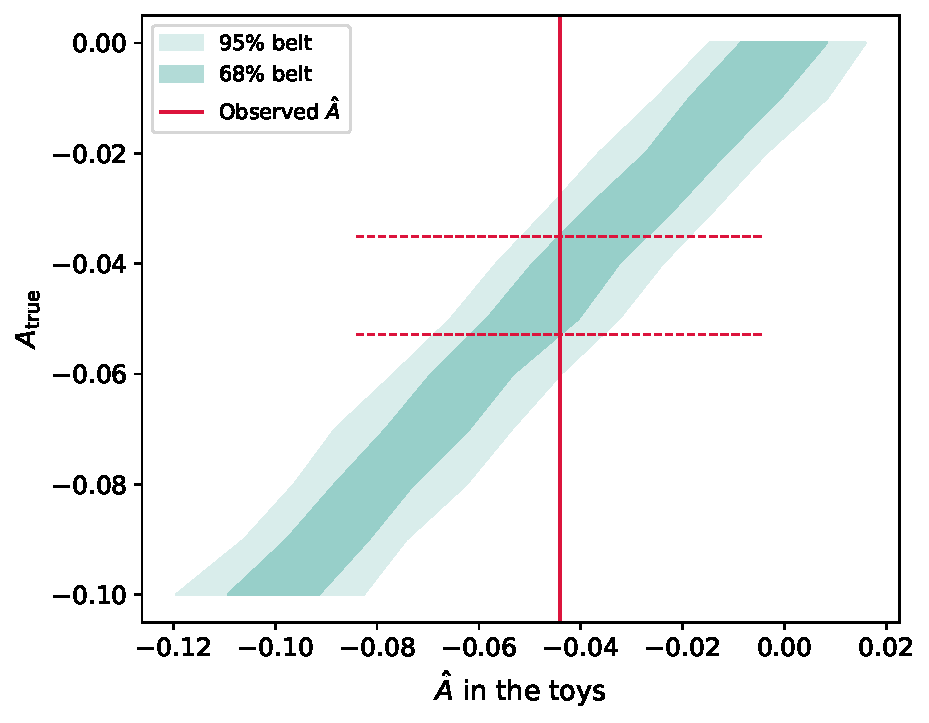
\includegraphics[width=0.4\textwidth]{figures/validation_neyman_belt.pdf}
\caption{Confidence belt of $\hat A$ from toy-MC experiments (central $68\%$ and $95\%$ ranges) as a function of $A_{\mathrm{true}}$; the vertical line is the observed $\hat A$ and the dashed lines the resulting $68\%$ interval.}
\label{fig:checks_belt}
\end{figure}
\begin{table}[!htbp]
\centering
\begin{tabular}{lccc}
\toprule
Bin & range [GeV] & $n$ & $\Araw$ \\
\midrule
$p_T$, 1 & $1.0$--$4.7$ & $6577$ & $-0.0563\pm0.0169$ \\
$p_T$, 2 & $4.7$--$8.2$ & $6577$ & $-0.0362\pm0.0141$ \\
$p_T$, 3 & $8.2$--$30.5$ & $6577$ & $-0.0452\pm0.0134$ \\
$p$, 1 & $26.7$--$78.1$ & $6577$ & $-0.0391\pm0.0139$ \\
$p$, 2 & $78.1$--$110.1$ & $6577$ & $-0.0475\pm0.0149$ \\
$p$, 3 & $110.1$--$288.5$ & $6577$ & $-0.0478\pm0.0153$ \\
\bottomrule
\end{tabular}
\caption{$\Araw$ (joint frequentist fit) in terciles of the transverse momentum and of the momentum of the $B$ candidate.}
\label{tab:checks_momentum}
\end{table}
\begin{figure*}[!tbp]
\centering
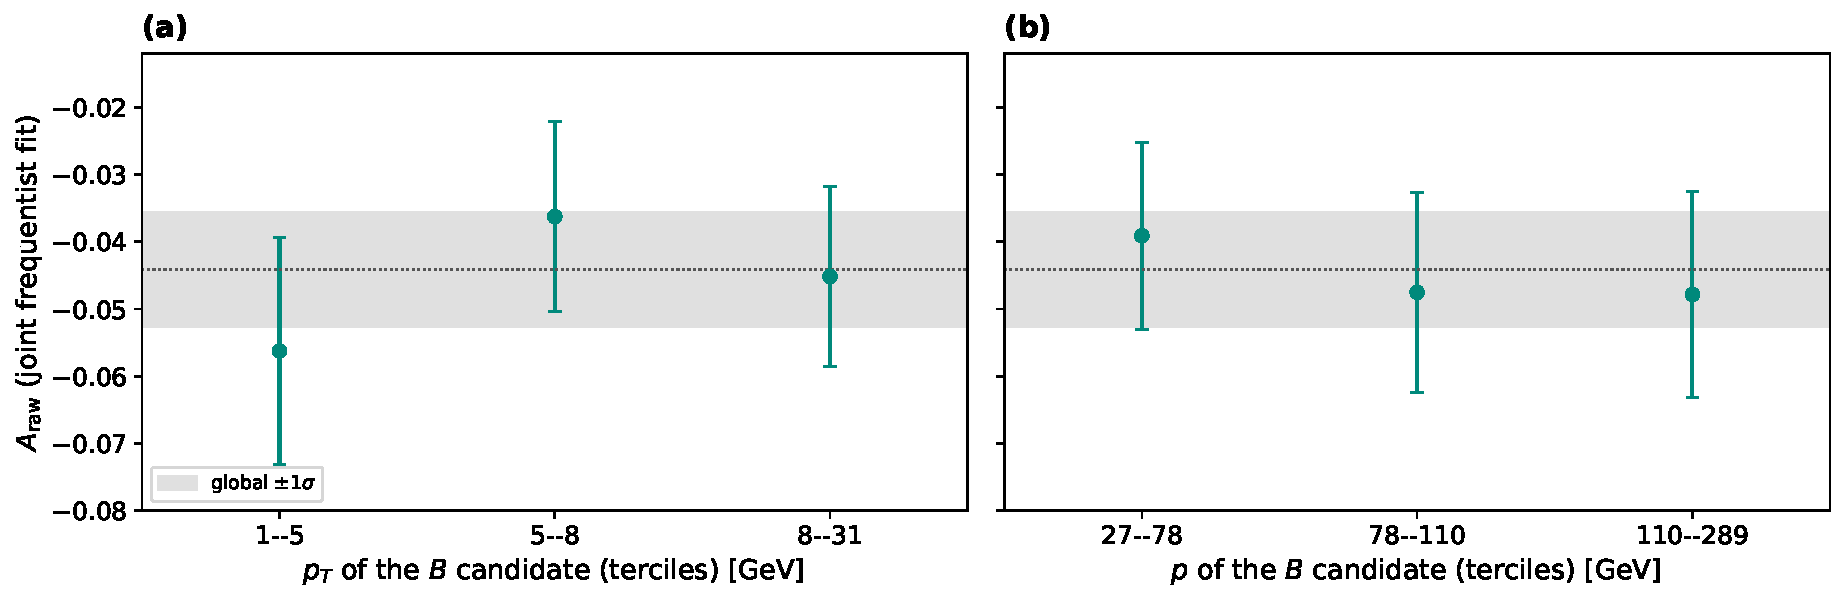
\includegraphics[width=0.85\textwidth]{figures/momentum_terciles.pdf}
\caption{$\Araw$ (joint frequentist fit) in terciles of (a) the transverse momentum and (b) the momentum of the $B$ candidate, with the global value and its $\pm1\sigma$ band; each bin has $6577$ candidates.}
\label{fig:momentum_terciles}
\end{figure*}

\FloatBarrier
\subsection{Uncertainties of the Twelve Parameters by Three Methods}
\label{sec:checks_covariance}
\emph{In short: the inverse of the Fisher information (Hesse), the bootstrap of the data and the posterior give the same standard deviations for $A$, $A_b$, $\mu$ and $\sigma$; the bootstrap differs for the two yields, because it keeps the total number of candidates fixed, and for the steep slope $\lambda_1^+$, which is weakly constrained.}
Table~\ref{tab:checks_covariance} lists the standard deviation of the twelve parameters from the Hesse matrix, the bootstrap and the posterior, and Fig.~\ref{fig:uncertainties_12} shows their ratios to the Hesse value.
\begin{table}[!htbp]
\centering
\begin{tabular}{lccc}
\toprule
Parameter & Hesse & Bootstrap & Posterior \\
\midrule
$A$ & $0.0085$ & $0.0085$ & $0.0085$ \\
$A_b$ & $0.0177$ & $0.0183$ & $0.0176$ \\
$N_s$ & $133$ & $72$ & $133$ \\
$N_b$ & $82$ & $72$ & $82$ \\
$\mu$ [MeV] & $0.159$ & $0.159$ & $0.161$ \\
$\sigma$ [MeV] & $0.141$ & $0.150$ & $0.138$ \\
$\lambda_1^+$ & $0.0077$ & $0.0057$ & $0.0078$ \\
$\lambda_2^+$ & $0.00028$ & $0.00030$ & $0.00029$ \\
$f_+$ & $0.028$ & $0.029$ & $0.030$ \\
$\lambda_1^-$ & $0.0047$ & $0.0043$ & $0.0047$ \\
$\lambda_2^-$ & $0.00040$ & $0.00038$ & $0.00039$ \\
$f_-$ & $0.039$ & $0.036$ & $0.037$ \\
\bottomrule
\end{tabular}
\caption{Standard deviation of the parameters of the nominal fit from the Hesse matrix, from the bootstrap of the data and from the posterior.}
\label{tab:checks_covariance}
\end{table}
\begin{figure*}[!tbp]
\centering
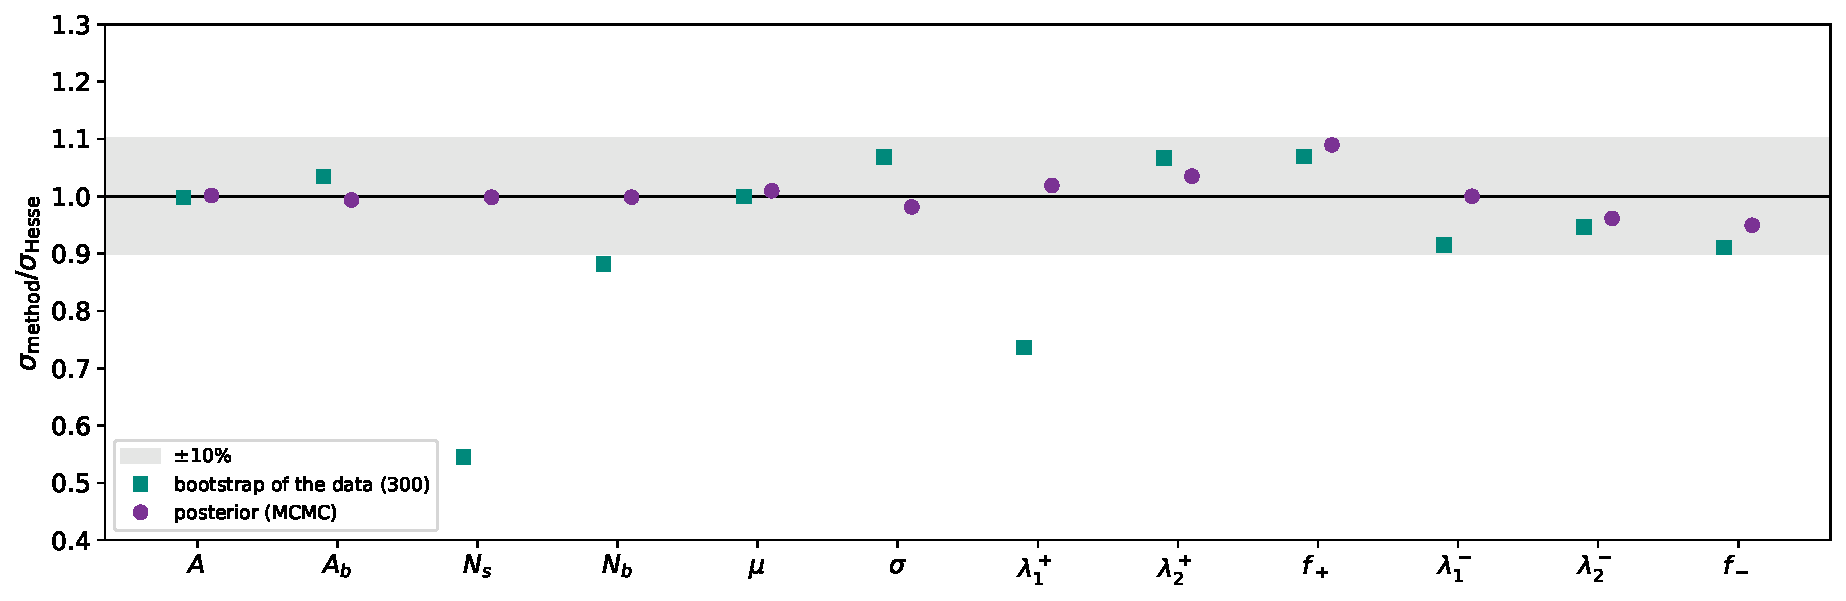
\includegraphics[width=0.85\textwidth]{figures/uncertainties_12.pdf}
\caption{Standard deviation of the twelve parameters of the nominal fit from the bootstrap of the data ($300$ replicas) and from the posterior, divided by the Hesse uncertainty; the band is $\pm10\%$.}
\label{fig:uncertainties_12}
\end{figure*}

\FloatBarrier
\subsection{Starting Values and Weakly Constrained Parameters}
\label{sec:checks_multistart}
\emph{In short: $29$ of $30$ fits from random starting points reach the same minimum; the steep-background fraction is the weakly constrained direction, as the long chain of the Bayesian fit already showed.}

\FloatBarrier
\section{Bayesian Analysis}
\label{app:ext_bayes}
\emph{In short: the sampling and the posterior summaries behind Sec.~\ref{sec:bayesian}, the Bayes factors with their derivation, the model-adequacy and robustness checks, the toy-MC coverage of the credible interval and the alternative sampler.}
\FloatBarrier
\subsection{Sampling the Posterior}
\label{app:theory}
\emph{In short: Metropolis-Hastings accepts a proposal with a ratio that satisfies detailed balance; the affine-invariant ensemble move samples correlated posteriors without tuning, and $N/\tau$ is the effective length of a chain.}

\FloatBarrier
\subsection{Posterior Summaries and Model Comparison}
\emph{In short: equal-tailed and HPD intervals, the Jeffreys scale for Bayes factors, the Ockham effect of the prior width and the definition of the posterior predictive $p$-value.}

\FloatBarrier
\subsection{Flat Priors and the Evidence}
\emph{In short: a flat prior is not invariant under reparametrization, but with $\sim2\times10^4$ events the posterior is dominated by the likelihood; the evidence is a constant that neither the MCMC nor the Savage-Dickey ratio needs.}

\FloatBarrier
\subsection{Sampling and Convergence Diagnostics}
\emph{In short: $32$ walkers for $25{,}000$ steps give $N/\tau\geq113$ autocorrelation times for every parameter, and runs started over the whole prior box converge to the same single mode.}

\FloatBarrier
\subsection{Trace Plots of the Walkers}
\label{sec:appendix}
\emph{In short: walkers started over the whole prior box converge to the same mode.}
Figure~\ref{fig:bayes_trace} shows the trace of the 32 walkers started over the whole prior box, for $A$, $N_s$, $\sigma$ and $f_+$.
\begin{figure*}[!tbp]
\centering
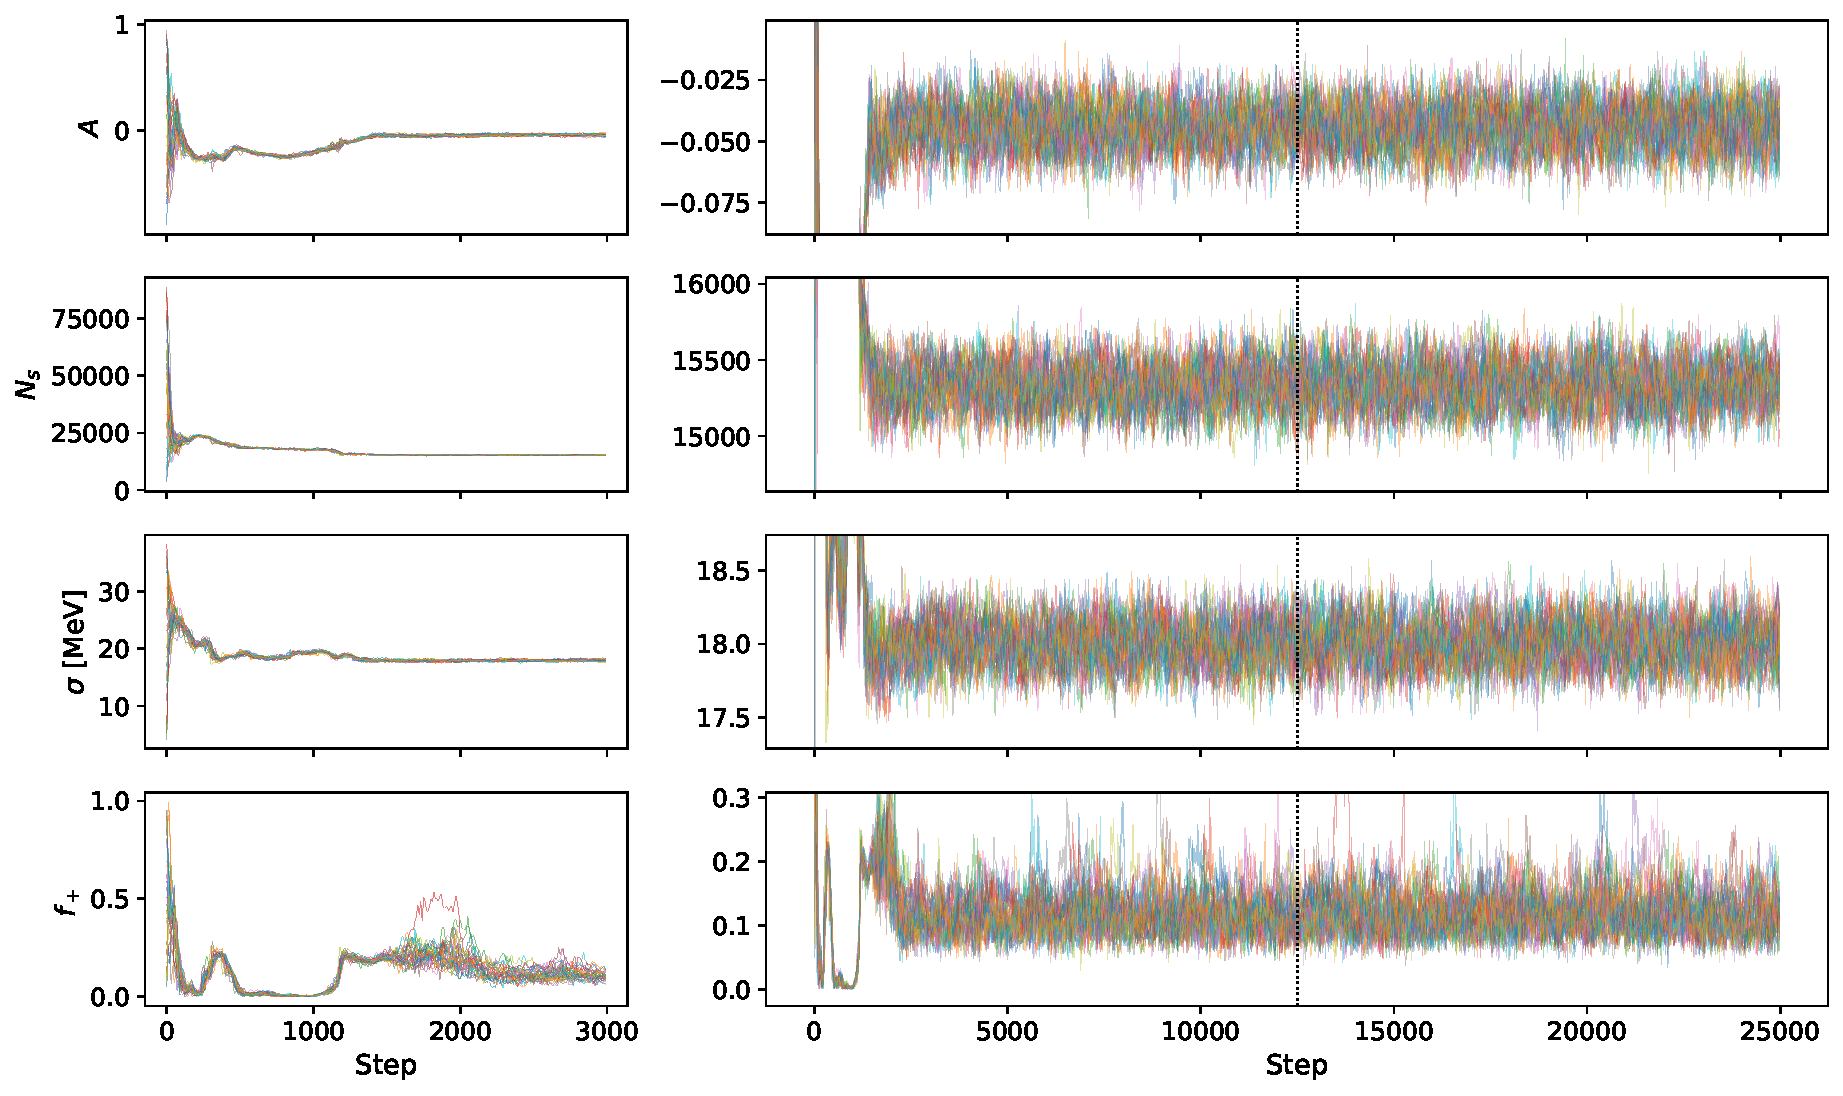
\includegraphics[width=0.75\textwidth]{figures/bayes_nominal_trace.pdf}
\caption{Trace plot of the nominal fit with the 32 walkers initialized uniformly over the prior box (one line per walker, every 10th step), for $A$, $N_s$, $\sigma$ and the steep-background fraction $f_+$. Left: first 3000 steps, full range; right: whole chain, zoomed on the posterior. The first half of the chain (dotted line) is discarded as burn-in.}
\label{fig:bayes_trace}
\end{figure*}

\FloatBarrier
\subsection{Posterior of the Raw Asymmetry}
\emph{In short: $\Araw=-0.0443$ with $68\%$ and $95\%$ intervals $[-0.0528,-0.0358]$ and $[-0.0608,-0.0276]$; the posterior is Gaussian, so equal-tailed and highest-density intervals coincide and its mode is the maximum-likelihood estimate.}

\FloatBarrier
\subsection{Equal-Tailed and Highest-Posterior-Density Intervals}
\label{sec:checks_hpd}
\emph{In short: for $A$ and $A_b$ the two kinds of $68\%$ interval coincide; they differ for the skewed parameters, whose highest-posterior-density interval is shifted towards the mode.}
Table~\ref{tab:checks_hpd} compares the equal-tailed and highest-posterior-density $68\%$ intervals and gives the skewness of each marginal posterior.
\begin{table}[!htbp]
\centering
\resizebox{\ifdim\width>\linewidth\linewidth\else\width\fi}{!}{\begin{tabular}{lcccc}
\toprule
Parameter & median & equal-tailed & HPD & skewness \\
\midrule
$A$ & $-0.0442$ & $[-0.0529,-0.0358]$ & $[-0.0525,-0.0355]$ & $+0.01$ \\
$A_b$ & $-0.0400$ & $[-0.0575,-0.0224]$ & $[-0.0575,-0.0225]$ & $+0.01$ \\
$f_+$ & $0.114$ & $[0.089,0.145]$ & $[0.084,0.138]$ & $+0.90$ \\
$f_-$ & $0.209$ & $[0.174,0.248]$ & $[0.168,0.241]$ & $+0.33$ \\
$\lambda_1^+$ [MeV$^{-1}$] & $0.0350$ & $[0.0281,0.0431]$ & $[0.0274,0.0423]$ & $+0.52$ \\
\bottomrule
\end{tabular}}
\caption{Equal-tailed and highest-posterior-density $68\%$ intervals and skewness of the marginal posteriors.}
\label{tab:checks_hpd}
\end{table}

\FloatBarrier
\subsection{Savage--Dickey Ratio}
\label{sec:appendix_sd}
\emph{In short: the Bayes factor of $A=0$ is the ratio of the posterior and prior densities at $A=0$, with no integral over the twelve parameters.}

\FloatBarrier
\subsection{Bayes Factor of $A=0$}
\emph{In short: the Savage-Dickey ratio with the Gaussian approximation of the posterior gives $BF_{01}\approx1.1\times10^{-4}$ ($BF_{10}\approx9\times10^3$), decisive evidence against $A=0$ that scales with the prior width.}

\FloatBarrier
\subsection{Bayes Factor of the Background Asymmetry}
\emph{In short: $A_b=-0.040\pm0.018$ is $2.3$ standard deviations from zero, yet $BF_{01}\approx3.5$ favors $A_b=0$ (Ockham factor); $A_b$ is kept free in the nominal model.}

\FloatBarrier
\subsection{Savage--Dickey Densities of the Parameters}
\label{app:sd_densities}
\emph{In short: the posterior and prior densities at the null value, which give the Bayes factors of the main text.}
Figure~\ref{fig:bayes_sd} shows the posterior and prior densities of $A$ and $A_b$, whose ratio at zero is the Bayes factor.
\begin{figure*}[!tbp]
\centering
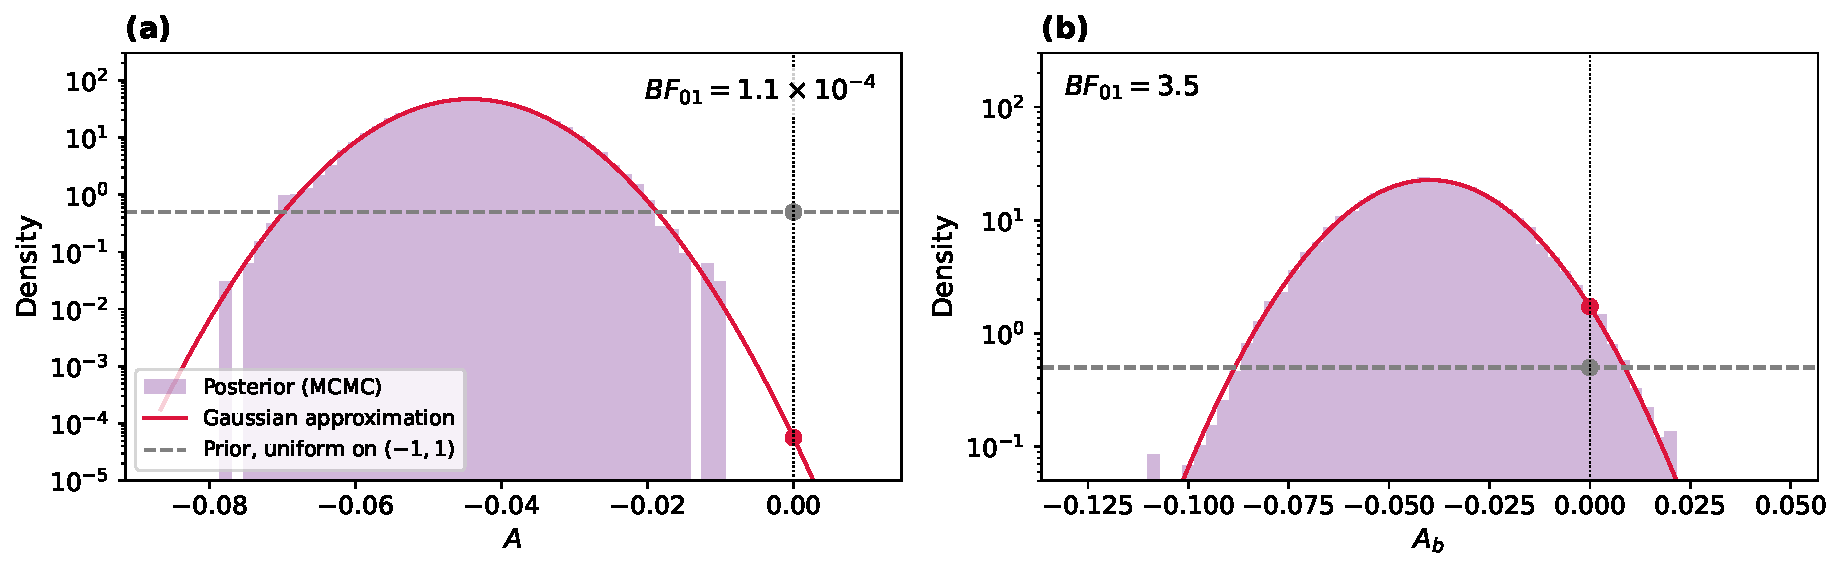
\includegraphics[width=0.75\textwidth]{figures/bayes_nominal_savage_dickey.pdf}
\caption{Savage-Dickey ratio for (a) $A$ and (b) $A_b$: marginal posterior (histogram of the chain and Gaussian approximation) and prior density, logarithmic scale. The Bayes factor $BF_{01}$ is the ratio of the two densities at zero (dots). For $A$ the posterior density at zero is $10^{-4}$ times the prior one; for $A_b$, $2.3$ standard deviations from zero, it is higher than the prior density, and the data favor $A_b=0$.}
\label{fig:bayes_sd}
\end{figure*}

\FloatBarrier
\subsection{Priors and Bayes Factors}
\label{sec:checks_prior}
\emph{In short: no change of the prior on the nuisance parameters or of its parametrization moves $A$ by more than $0.0002$; the Bayes factor of $A=0$ scales with the prior width, and the evidence computed by direct integration agrees in order of magnitude with the Savage-Dickey ratio.}
Table~\ref{tab:checks_prior} gives the posterior of $A$ under the alternative priors, with the effective sample size of each reweighting.
\begin{table}[!htbp]
\centering
\resizebox{\ifdim\width>\linewidth\linewidth\else\width\fi}{!}{\begin{tabular}{lccc}
\toprule
Prior & $A$ (median) & $68\%$ interval & ESS \\
\midrule
Nominal (uniform) & $-0.0442$ & $[-0.0529,-0.0358]$ & $20000$ \\
Log-uniform $N_s$, $N_b$ & $-0.0442$ & $[-0.0529,-0.0358]$ & $19993$ \\
Log-uniform slopes & $-0.0440$ & $[-0.0528,-0.0356]$ & $12306$ \\
Uniform in $1/\lambda$ & $-0.0444$ & $[-0.0526,-0.0360]$ & $153$ \\
Flat in $(N_s^+,N_s^-)$ & $-0.0442$ & $[-0.0529,-0.0358]$ & $19999$ \\
Flat in $(N_s^\pm)$ and $(N_b^\pm)$ & $-0.0442$ & $[-0.0529,-0.0358]$ & $19993$ \\
\bottomrule
\end{tabular}}
\caption{Posterior of $A$ under alternative priors, by importance reweighting of the chain; ESS: effective sample size of the $20{,}000$ thinned samples.}
\label{tab:checks_prior}
\end{table}

\FloatBarrier
\subsection{Model Adequacy: Goodness of Fit and Posterior Predictive Check}
\label{sec:bayes_gof}
\emph{In short: the model does not reach $\chi^2/\mathrm{ndof}\approx1$ ($164.1/88$), mainly because the signal tails are heavier than a Gaussian, but $\Araw$ changes by only $-0.0002$ with a Crystal Ball signal.}
Table~\ref{tab:gof} compares $\Araw$ and the goodness of fit of the nominal model with those of the alternative signal and background models, and Fig.~\ref{fig:bayes_ppc} shows the posterior predictive check of the $\chi^2$ and of the counting asymmetry in the fit window and in the sidebands.
\begin{table}[!htbp]
\centering
\begin{tabular}{lccc}
\toprule
Model & $\Araw$ & $\chi^2$/ndof & $p$ \\
\midrule
Nominal & $-0.0443$ & $164.1/88$ & $2\times10^{-6}$ \\
Crystal Ball signal & $-0.0445$ & $131.0/86$ & $1\times10^{-3}$ \\
$\mu$, $\sigma$ per charge & $-0.0443$ & $164.2/86$ & $8\times10^{-7}$ \\
Shared bkg.\ shape & $-0.0480$ & $174.1/91$ & $4\times10^{-7}$ \\
Symmetric bkg.\ ($A_b=0$) & $-0.0471$ & $169.8/89$ & $5\times10^{-7}$ \\
Single exponential & $-0.0480$ & $297.7/92$ & $2\times10^{-23}$ \\
\bottomrule
\end{tabular}
\caption{$\Araw$ (posterior median) and goodness of fit of the nominal model (Gaussian signal, double exponential per charge) and of the alternative signal and background models, same data and window.}
\label{tab:gof}
\end{table}
\begin{figure*}[!tbp]
\centering
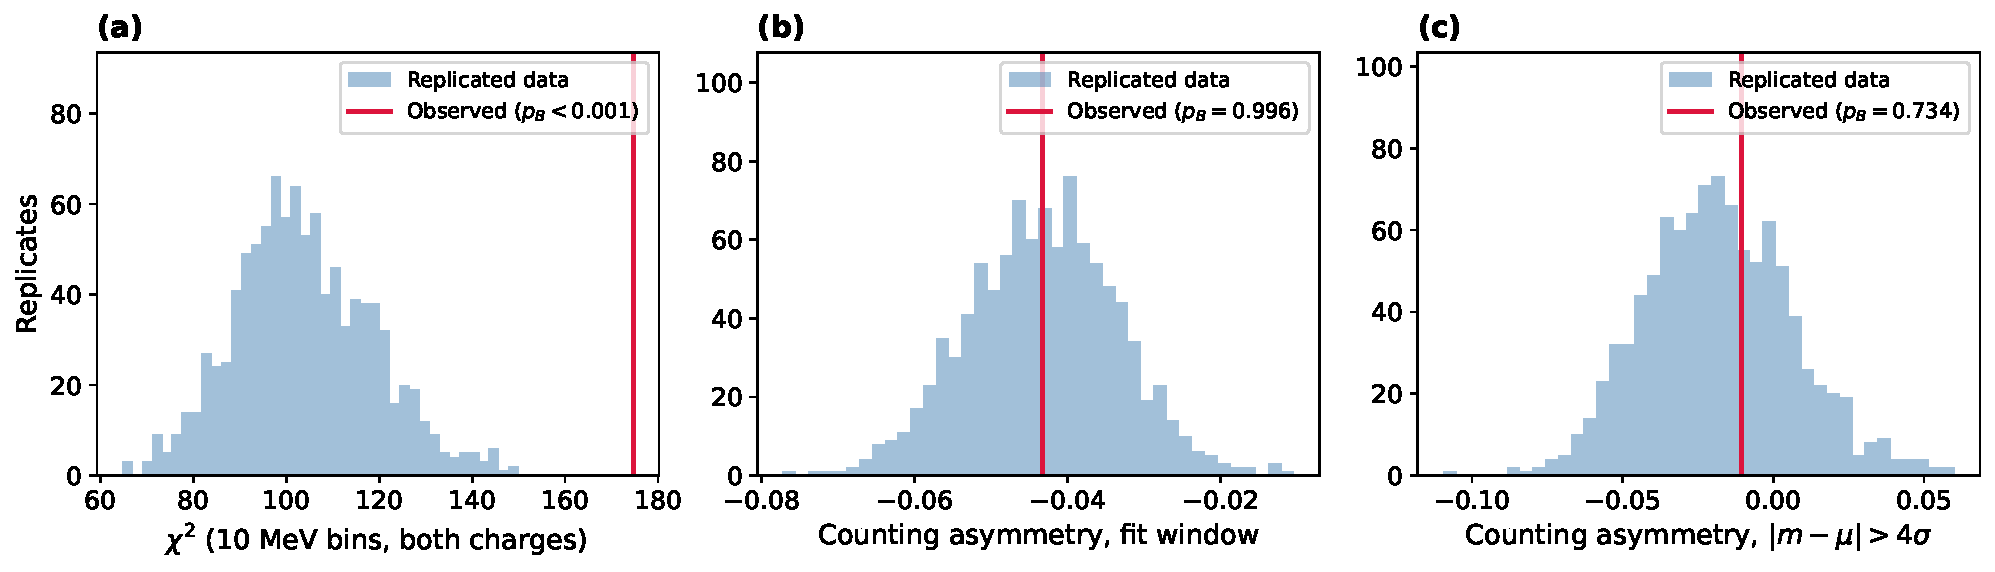
\includegraphics[width=0.75\textwidth]{figures/bayes_nominal_ppc.pdf}
\caption{Posterior predictive check: distributions of three discrepancies over $1000$ datasets replicated from posterior draws, compared with the observed values. (a) binned $\chi^2$; (b) and (c) counting asymmetry of the fit window and of the sidebands.}
\label{fig:bayes_ppc}
\end{figure*}

\FloatBarrier
\subsection{Posterior Predictive Check with Statistics Not Fitted by the Model}
\label{sec:checks_ppc}
\emph{In short: the asymmetry in slices of the mass, which the model predicts, is reproduced ($p_B=0.67$), and the difference between the $\chi^2$ of the two charges is at the edge of the replicas ($p_B=0.08$).}
Figure~\ref{fig:checks_ppc} shows the asymmetry in slices of the mass against the model (a) and the replicas of the two statistics against their observed values (b, c).
\begin{figure*}[!tbp]
\centering
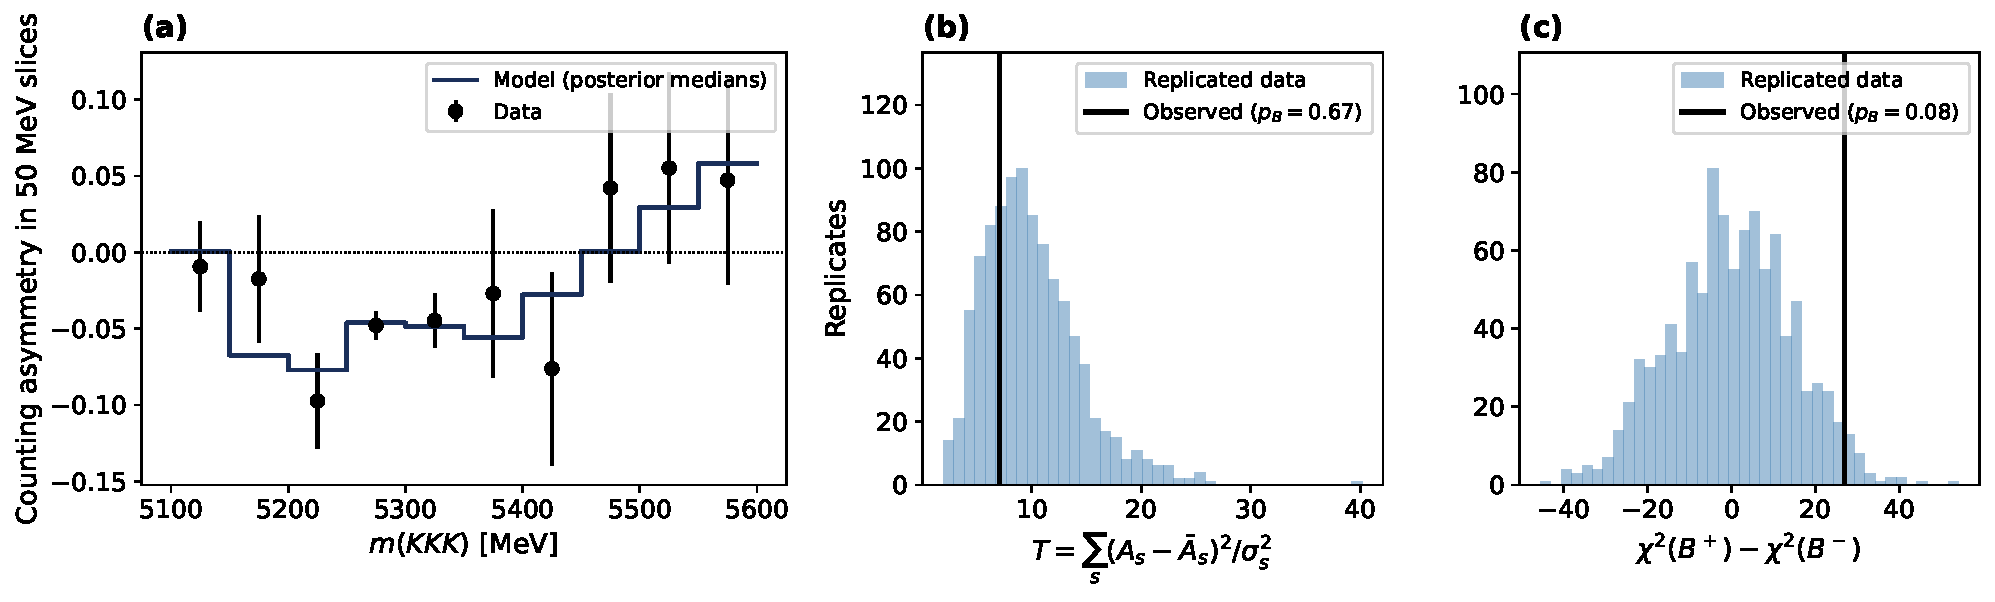
\includegraphics[width=0.75\textwidth]{figures/validation_ppc_unfitted.pdf}
\caption{(a) Counting asymmetry in slices of $50\,\MeV$ of the mass, data and model. (b) Distribution of $T=\sum_s(A_s-\bar A_s)^2/\sigma_s^2$ over $1000$ replicas and observed value. (c) The same for $\chi^2(B^+)-\chi^2(B^-)$.}
\label{fig:checks_ppc}
\end{figure*}

\FloatBarrier
\subsection{Robustness Checks: Polarity, Prior and Charm Vetoes}
\label{sec:bayes_checks}
\emph{In short: $\Araw$ agrees between the two magnet polarities ($0.7\sigma$) and does not depend on the prior; the $D^0$ veto moves it by $2.3$ times the expected statistical spread.}
Figure~\ref{fig:bayes_magnet} shows the posterior of $\Araw$ for the two magnet polarities and for the combined sample.
\begin{figure}[!htbp]
\centering
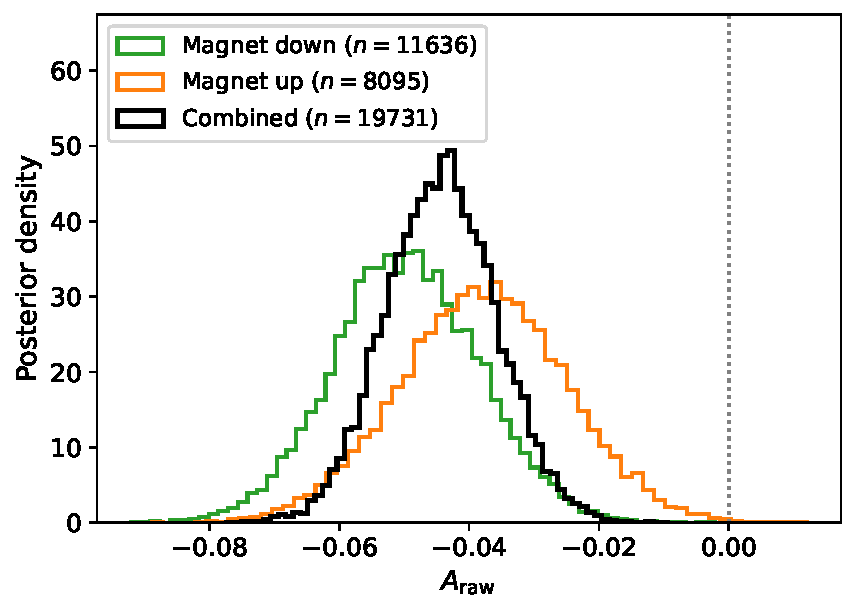
\includegraphics[width=0.4\textwidth]{figures/bayes_nominal_magnet.pdf}
\caption{Posterior of $\Araw$ for the magnet-down, magnet-up and combined samples.}
\label{fig:bayes_magnet}
\end{figure}

\FloatBarrier
\subsection{Toy-MC Coverage Validation}
\label{sec:bayes_toymc}
\emph{In short: $200$ toy-MC experiments give coverage $0.65\pm0.03$ ($68\%$) and $0.93\pm0.02$ ($95\%$), consistent with nominal, with unbiased estimates and pulls of width $1.04$.}
Figure~\ref{fig:bayes_toys} shows the pulls (a) and the coverage of the $68\%$ and $95\%$ intervals (b).
\begin{figure}[!htbp]
\centering
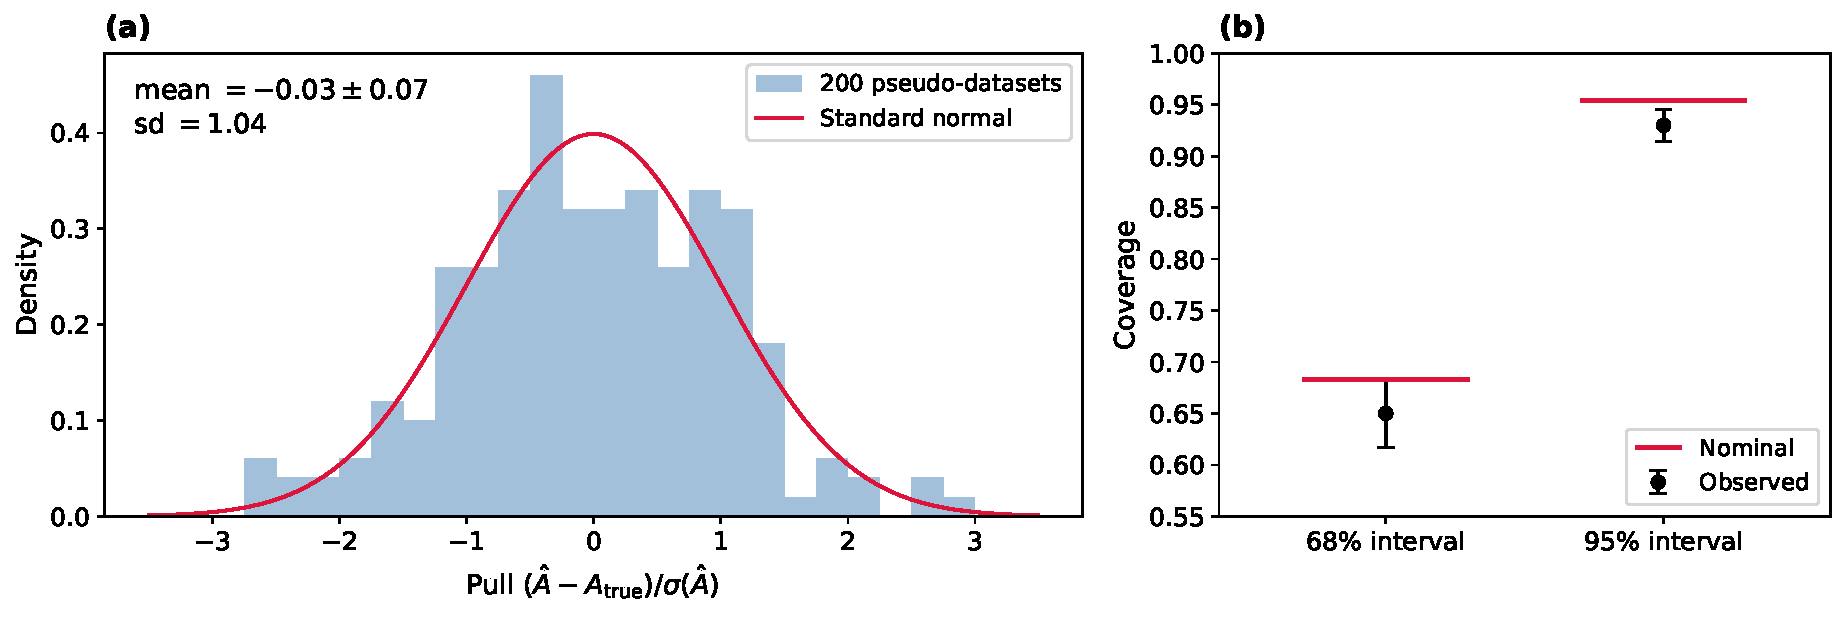
\includegraphics[width=0.4\textwidth]{figures/bayes_nominal_toys.pdf}
\caption{Toy-MC validation, 200 toy-MC datasets. (a) Pulls $(\hat A-A_{\mathrm{true}})/\sigma(\hat A)$, with $\hat A$ and $\sigma(\hat A)$ the posterior median and standard deviation of each replica, compared with a standard normal. (b) Fraction of replicas whose 68\% and 95\% credible intervals contain the injected value, with binomial uncertainties, and the nominal coverage.}
\label{fig:bayes_toys}
\end{figure}

\FloatBarrier
\subsection{Metropolis-Hastings Sampler and Published Likelihood}
\label{sec:checks_mh}
\emph{In short: an own Metropolis-Hastings sampler reproduces the posterior of the ensemble sampler, and the profile likelihood is given in a table, so that the result can be combined with others.}
Table~\ref{tab:checks_qa} gives the profile likelihood ratio of the nominal fit and its Minos intervals.
\begin{table}[!htbp]
\centering
\resizebox{\ifdim\width>\linewidth\linewidth\else\width\fi}{!}{\begin{tabular}{r|ccccccccc}
\toprule
$A$ & $-0.08$ & $-0.07$ & $-0.06$ & $-0.05$ & $-0.04$ & $-0.03$ & $-0.02$ & $-0.01$ & $+0.00$ \\
$q(A)$ & $17.9$ & $9.3$ & $3.5$ & $0.5$ & $0.2$ & $2.8$ & $8.1$ & $16.1$ & $27.0$ \\
\bottomrule
\end{tabular}}
\caption{Profile likelihood ratio $q(A)=-2\Delta\ln L$ of the nominal fit (other parameters profiled); minimum at $-0.0441$, Minos intervals $[-0.0526,-0.0356]$ ($68\%$) and $[-0.0607,-0.0275]$ ($95\%$).}
\label{tab:checks_qa}
\end{table}

\FloatBarrier
\section{Systematic Uncertainties}
\label{app:syst}
\emph{In short: every fit of the nominal model and of its variants with both methods, the variants and the rule that combines them, and the validation of that rule on nested samples.}
\FloatBarrier
\subsection{All Fits of the Nominal Model and of Its Variants}
\label{sec:syst_tables}
\emph{In short: the Bayesian and frequentist results of every variant and cross-check side by side.}
Table~\ref{tab:bayes_all} lists every fit, Bayesian and frequentist, of the nominal model and of its variants.
\begin{table*}[!tbp]
\centering
\begin{tabular}{lrccc|c}
\toprule
Fit & $n$ & $\Araw$ Bayesian (median) & 68\% CI & $\chi^2$/ndof & $\Araw$ frequentist \\
\midrule
Nominal & $19731$ & $-0.0443$ & $[-0.0528,-0.0358]$ & $164.1/88$ & $-0.0441\pm0.0085$ \\
\multicolumn{6}{l}{\emph{Systematic variants (Sec.~\ref{sec:syst})}} \\
Window $[5050,5600]$ & $21164$ & $-0.0446$ & $[-0.0531,-0.0362]$ & $217.4/98$ & $-0.0445\pm0.0085$ \\
Window $[5150,5600]$ & $18566$ & $-0.0444$ & $[-0.0528,-0.0359]$ & $141.5/78$ & $-0.0446\pm0.0088$$^\dagger$ \\
Window $[5100,5450]$ & $19004$ & $-0.0440$ & $[-0.0524,-0.0357]$ & $136.9/58$ & $-0.0442\pm0.0085$ \\
Window $[5100,5700]$ & $20191$ & $-0.0456$ & $[-0.0540,-0.0373]$ & $200.2/108$ & $-0.0455\pm0.0085$ \\
Single exponential & $19731$ & $-0.0480$ & $[-0.0564,-0.0395]$ & $297.7/92$ & $-0.0481\pm0.0085$ \\
Background shape shared & $19731$ & $-0.0480$ & $[-0.0564,-0.0397]$ & $174.1/91$ & $-0.0481\pm0.0083$ \\
Symmetric background & $19731$ & $-0.0471$ & $[-0.0552,-0.0388]$ & $169.8/89$ & $-0.0472\pm0.0084$ \\
Crystal Ball signal & $19731$ & $-0.0445$ & $[-0.0529,-0.0363]$ & $131.0/86$ & $-0.0447\pm0.0085$ \\
$\mu,\sigma$ per charge & $19731$ & $-0.0443$ & $[-0.0527,-0.0356]$ & $164.2/86$ & $-0.0442\pm0.0087$ \\
$\texttt{ProbK}>0.4$ & $26553$ & $-0.0474$ & $[-0.0550,-0.0399]$ & $175.6/88$ & $-0.0473\pm0.0076$ \\
$\texttt{ProbK}>0.6$ & $13981$ & $-0.0385$ & $[-0.0482,-0.0289]$ & $145.0/88$ & $-0.0384\pm0.0099$ \\
$\texttt{ProbPi}<0.4$ & $17984$ & $-0.0421$ & $[-0.0506,-0.0333]$ & $150.1/88$ & $-0.0421\pm0.0088$ \\
$\texttt{ProbPi}<0.6$ & $20953$ & $-0.0446$ & $[-0.0529,-0.0366]$ & $159.0/88$ & $-0.0448\pm0.0083$ \\
\multicolumn{6}{l}{\emph{Cross-checks (Secs.~\ref{sec:bayes_mcmc}, \ref{sec:bayes_checks})}} \\
Dispersed start, run 1 & $19731$ & $-0.0446$ & $[-0.0529,-0.0360]$ & $164.1/88$ & -- \\
Dispersed start, run 2 & $19731$ & $-0.0442$ & $[-0.0528,-0.0356]$ & $164.1/88$ & -- \\
Magnet down & $11636$ & $-0.0497$ & $[-0.0607,-0.0386]$ & $153.1/88$ & -- \\
Magnet up & $8095$ & $-0.0378$ & $[-0.0507,-0.0251]$ & $150.3/88$ & -- \\
Narrow prior, $A\in(-0.3,0.3)$ & $19731$ & $-0.0443$ & $[-0.0528,-0.0358]$ & $164.1/88$ & -- \\
$D^0$ veto & $18744$ & $-0.0496$ & $[-0.0584,-0.0409]$ & $159.1/88$ & $-0.0493\pm0.0087$ \\
$D^0$, $J/\psi$, $\chi_{c0}$ vetoes & $16367$ & $-0.0423$ & $[-0.0516,-0.0329]$ & $140.1/88$ & $-0.0421\pm0.0094$ \\
\bottomrule
\end{tabular}
\caption{All fits of the nominal model and of its variants: number of candidates, Bayesian posterior median and 68\% credible interval of $\Araw$, binned goodness of fit ($10\,\MeV$ bins), and frequentist estimate with its Hesse uncertainty (Sec.~\ref{sec:frequentist}; fitted on the same candidates; the cross-checks of the Bayesian fits that have no frequentist counterpart in this work are marked --). $^\dagger$ Uncertainty scaled from the number of events, since the Hesse matrix of that fit is not accurate. Every fit uses 32 walkers and $25{,}000$ steps.}
\label{tab:bayes_all}
\end{table*}

\FloatBarrier
\subsection{List of the Variants}
\emph{In short: thirteen variants of the nominal choices, in four groups (window, background, signal, preselection), fitted by both methods on exactly the same candidates.}

\FloatBarrier
\subsection{Combination Rule}
\emph{In short: a variant that changes the sample counts only if its shift exceeds $\sigma_B$; variants rejected by the data are excluded, the largest shift of each group is its uncertainty, and the groups are added in quadrature.}

\FloatBarrier
\subsection{Results and Particle-Identification Scan}
\emph{In short: the total systematic uncertainties are $0.0070$ (Bayesian) and $0.0072$ (frequentist), dominated by the preselection through the single variant $\texttt{ProbK}>0.6$ ($+0.0058$, $1.2\,\sigma_B$).}

\FloatBarrier
\subsection{Shifts of All Variants}
\label{app:syst_variants}
\emph{In short: the shifts of the Bayesian and frequentist fits coincide variant by variant; the preselection group dominates, and the single exponential, rejected by the data, is drawn open.}
Figure~\ref{fig:syst_variants} shows the shift of every variant for the two fits.
\begin{figure}[!htbp]
\centering
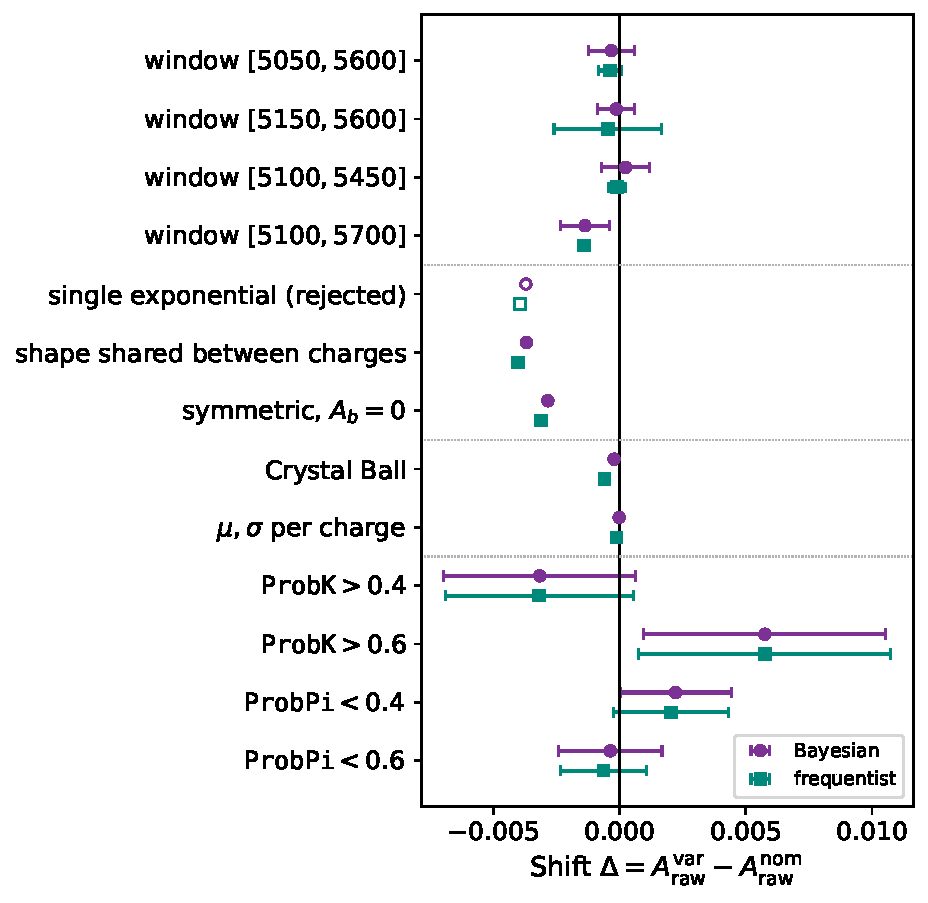
\includegraphics[width=0.4\textwidth]{figures/syst_variants.pdf}
\caption{Shift $\Delta=A_{\mathrm{raw}}^{\mathrm{var}}-A_{\mathrm{raw}}^{\mathrm{nom}}$ of every variant of the systematic study, Bayesian and frequentist fits; bars: expected spread $\sigma_B$ of a nested subsample (variants that change the sample only). Open symbols: variant rejected by the data. The dotted lines separate the groups (window, background, signal, preselection).}
\label{fig:syst_variants}
\end{figure}

\FloatBarrier
\subsection{Scan of the Particle-Identification Cuts}
\emph{In short: on the tight side the shift scatters around zero within $1.3\,\sigma_B$ and the pion requirement is flat; loosening $\texttt{ProbK}$ moves $\Araw$ monotonically, which supports the nominal requirement.}
Figure~\ref{fig:syst_pid_scan} shows the shift of $\Araw$ as the $\mathtt{ProbK}$ and $\mathtt{ProbPi}$ cuts are varied.
\begin{figure*}[!tbp]
\centering
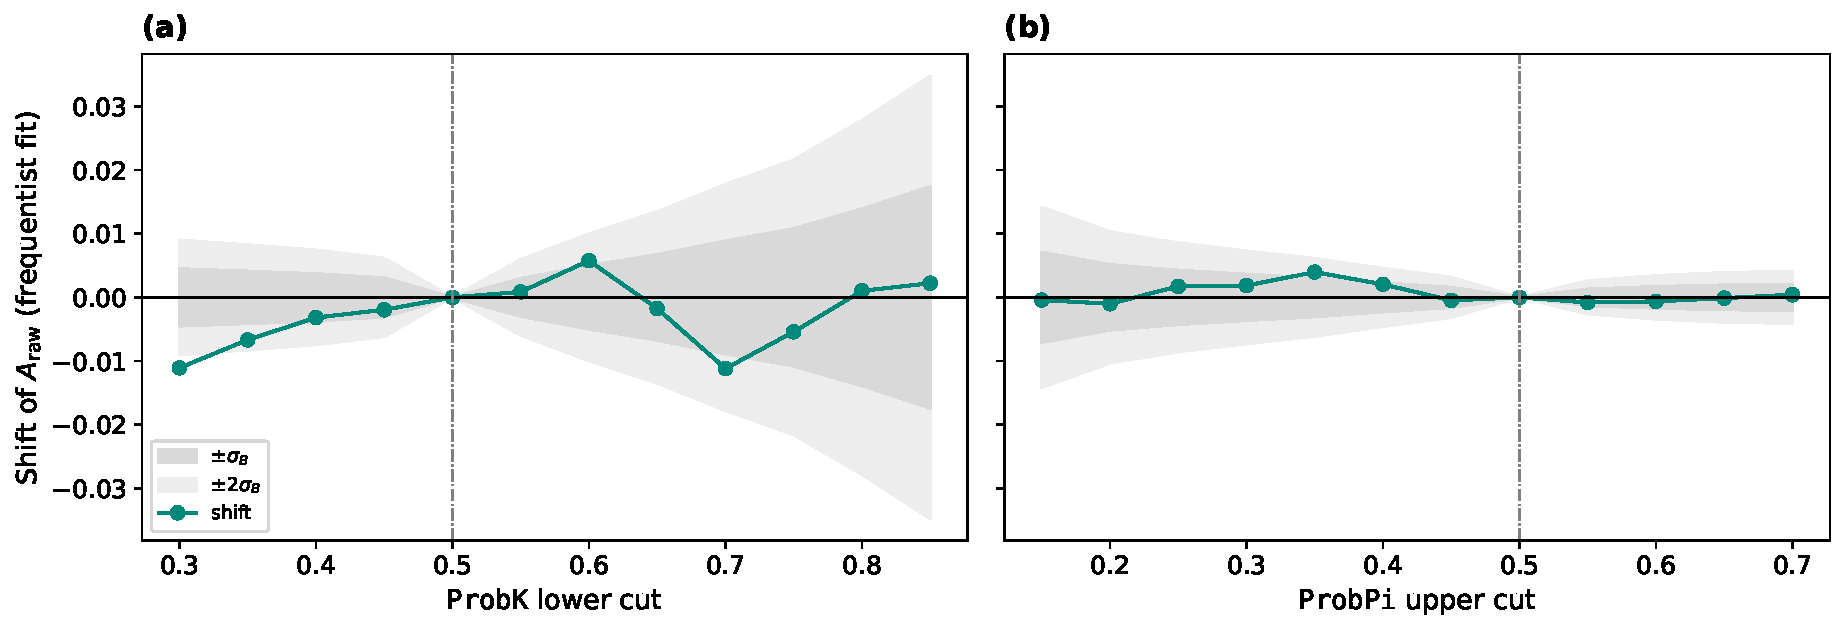
\includegraphics[width=0.85\textwidth]{figures/syst_pid_scan.pdf}
\caption{Shift of $\Araw$ (frequentist fit) as a function of (a) the $\mathtt{ProbK}$ lower cut and (b) the $\mathtt{ProbPi}$ upper cut, in steps of $0.05$, with the expected statistical spread of the nested sample ($\pm\sigma_B$ dark, $\pm2\sigma_B$ light; zero at the nominal cut, dash-dotted line). On the tight side of $\mathtt{ProbK}$ the points scatter around zero without trend and the pion requirement is flat; loosening $\mathtt{ProbK}$ moves $\Araw$ monotonically.}
\label{fig:syst_pid_scan}
\end{figure*}

\FloatBarrier
\subsection{Sensitivity of $\sigma_B$ to Differences between the Methods}
\emph{In short: $\sigma_B$ is the difference of two nearly equal uncertainties and is sensitive to small differences between the methods; a variant at the threshold can be classified differently without changing the result.}

\FloatBarrier
\subsection{Validation of the Rule for Nested Samples}
\label{sec:checks_barlow}
\emph{In short: the spread of the shift of $\hat A$ between a sample and its tighter-identification subsample is the one given by the quadrature difference of the uncertainties.}
Figure~\ref{fig:checks_barlow} shows the shift of $\hat A$ between the nominal sample and a tighter selection, divided by $\sigma_B$, in $300$ bootstrap replicas of the data.
\begin{figure*}[!tbp]
\centering
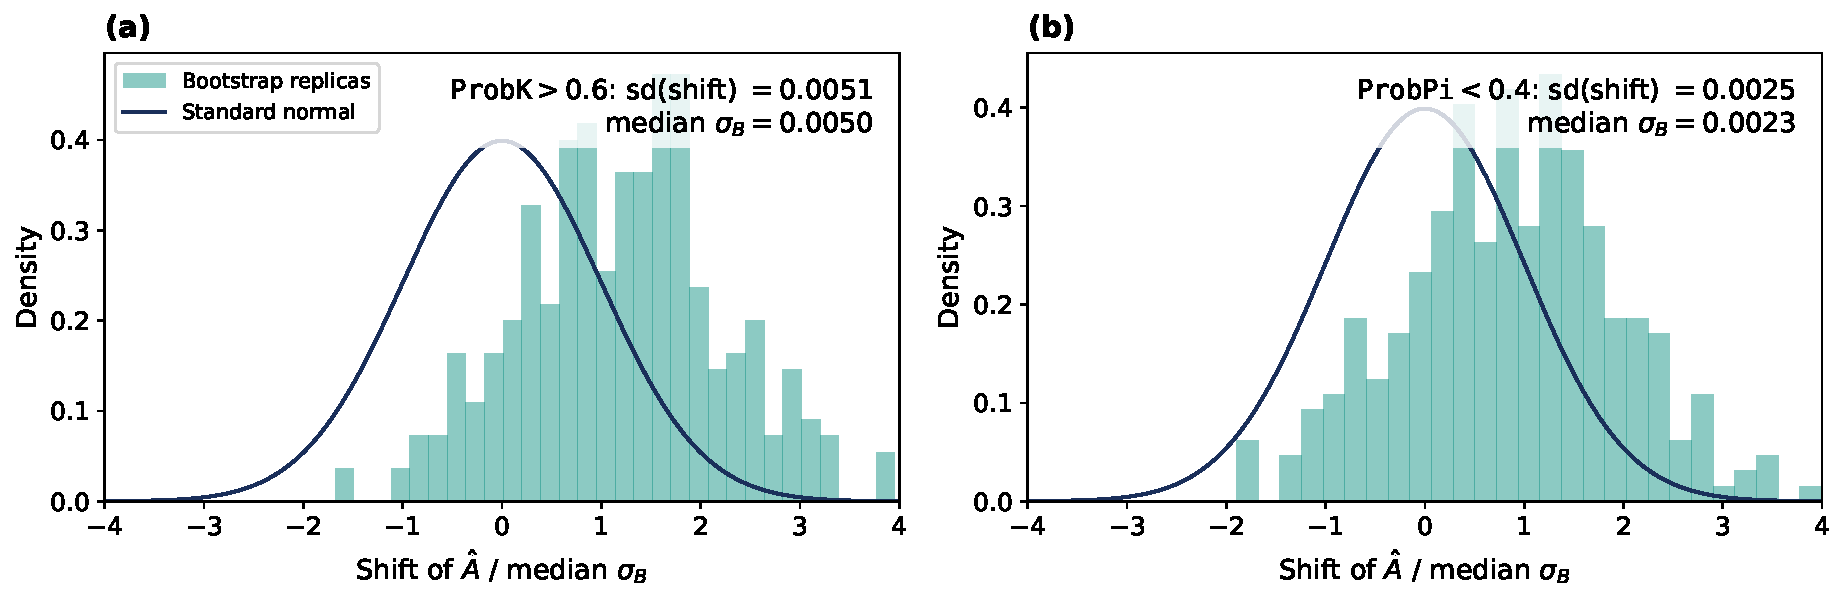
\includegraphics[width=0.75\textwidth]{figures/validation_barlow.pdf}
\caption{Shift of $\hat A$ between the nominal sample and a tighter selection, divided by the median $\sigma_B$, in $300$ bootstrap replicas of the data: (a) $\texttt{ProbK}>0.6$, (b) $\texttt{ProbPi}<0.4$, and standard normal distribution.}
\label{fig:checks_barlow}
\end{figure*}

\FloatBarrier
\subsection{Stability Scans of the Frequentist Fit: Numbers}
\emph{In short: the largest shifts are $0.0048$ over the grid of window edges and $0.0126$ over the grid of the two PID cuts, whose samples are smaller (mean uncertainty $0.0112$); the signal region moves $\Araw$ by $6\times10^{-5}$.}

\FloatBarrier
\section{Validation of the Estimator and of the Intervals}
\label{app:ext_valid}
\label{sec:appendix_checks}
\emph{In short: how the toy-MC experiments are generated, the bias, efficiency and coverage of the estimator, its asymptotic behavior, the size and power of the test of $A=0$ and the goodness of fit as a function of the binning.}
\FloatBarrier
\subsection{Generation of the Toy-MC Experiments}
\emph{In short: toy experiments are generated from the fitted model (Poisson yields, masses by the transformation method) and fitted with the nominal procedure: $1000$ at the fitted value and $300$ at each of four other values of $A$.}

\FloatBarrier
\subsection{Bias, Efficiency and Coverage}
\emph{In short: the bias is at most $0.0008$, the spread equals the Hesse uncertainty within $6\%$, and the coverage at the fitted value is $0.696\pm0.015$ and $0.954\pm0.007$.}

\FloatBarrier
\subsection{Asymptotic Behavior of the Estimator}
\label{sec:checks_scaling}
\emph{In short: with the number of candidates the bias tends to zero, the spread scales as $N^{-1/2}$ and the distribution of $\hat A$ becomes Gaussian, as the central limit theorem and the asymptotic properties of the maximum-likelihood estimate predict.}
Table~\ref{tab:checks_scaling} gives the bias, the spread, the skewness, the excess kurtosis and the Shapiro--Wilk $p$-value of $\hat A$ against the number of candidates.
\begin{table}[!htbp]
\centering
\resizebox{\ifdim\width>\linewidth\linewidth\else\width\fi}{!}{\begin{tabular}{rcccccc}
\toprule
$N$ & bias & sd$(\hat A)$ & sd$\cdot\sqrt N$ & skewness & ex.\ kurtosis & Shapiro $p$ \\
\midrule
$50$ & $-0.0085$ & $0.1611$ & $1.14$ & $-0.15$ & $+0.64$ & $0.03$ \\
$150$ & $-0.0051$ & $0.0920$ & $1.13$ & $+0.16$ & $+0.31$ & $0.59$ \\
$500$ & $-0.0022$ & $0.0501$ & $1.12$ & $-0.08$ & $+0.38$ & $0.52$ \\
$2000$ & $+0.0009$ & $0.0225$ & $1.01$ & $-0.20$ & $-0.20$ & $0.32$ \\
\bottomrule
\end{tabular}}
\caption{Distribution of the maximum-likelihood estimate of $A$ in $300$ toy-MC datasets of $N$ candidates (six-parameter model of Sec.~\ref{sec:bayes_minimal}).}
\label{tab:checks_scaling}
\end{table}

\FloatBarrier
\subsection{Size and Power of the Test of $A=0$}
\label{sec:validation_power}
\emph{In short: the test has the nominal size, the statistic $q(0)$ follows a $\chi^2$ distribution with one degree of freedom, and an asymmetry of $-0.02$ would be rejected at $3\sigma$ in one toy-MC experiment out of four.}
Figure~\ref{fig:validation_null} tests Wilks' theorem, and Fig.~\ref{fig:validation_injection} shows bias, spread and probability of rejecting $A=0$ at five injected asymmetries.
\begin{figure*}[!tbp]
\centering
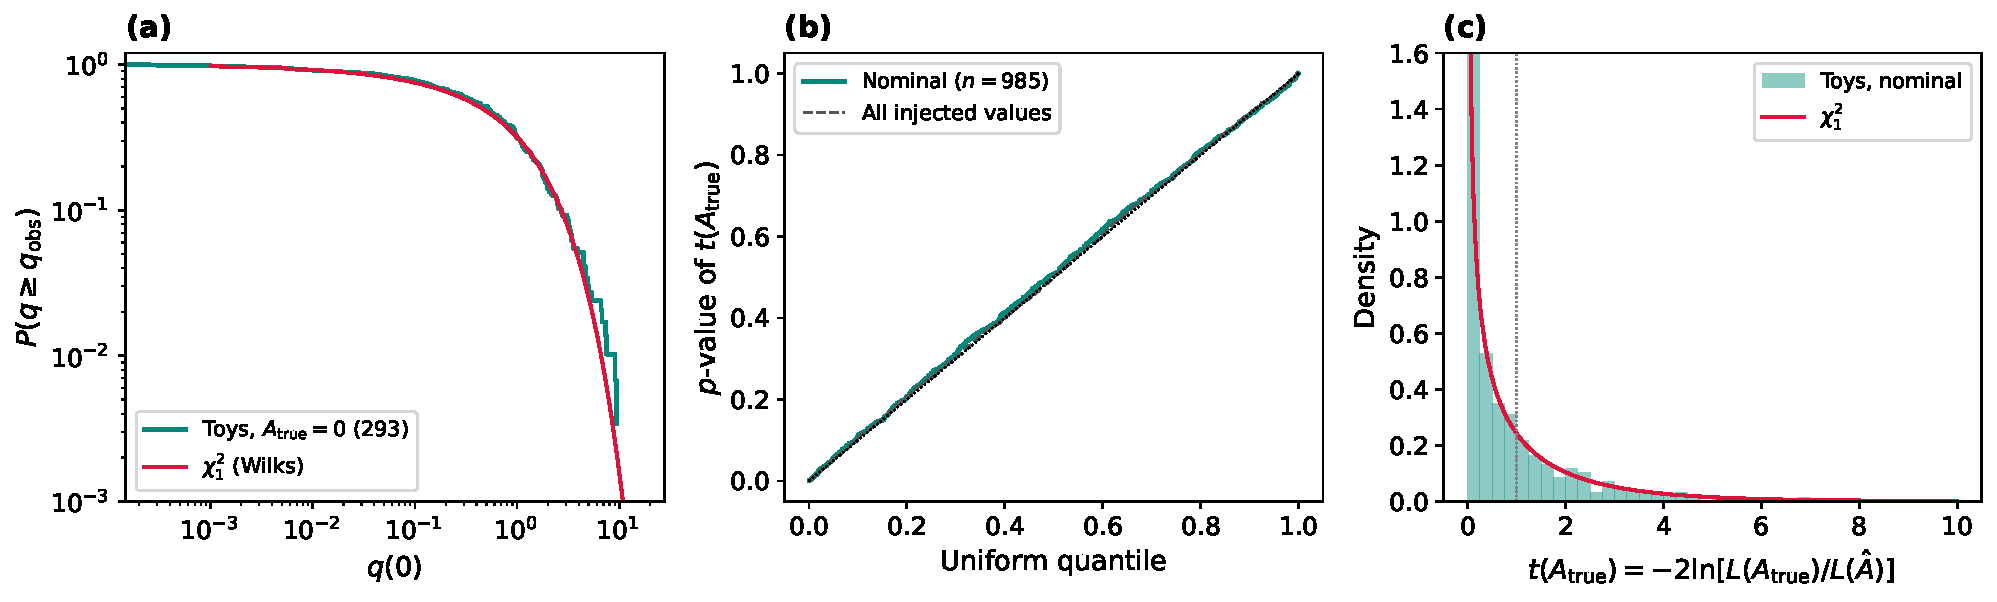
\includegraphics[width=0.75\textwidth]{figures/validation_null_wilks.pdf}
\caption{Toy-MC experiments, validity of Wilks' theorem. (a) Fraction of experiments with $q(0)$ above the observed value, for $A_{\mathrm{true}}=0$, compared with the $\chi^2_1$ distribution. (b) $p$-value of $t(A_{\mathrm{true}})$ against a uniform distribution, at the fitted value and pooled over the injected values. (c) Distribution of $t(A_{\mathrm{true}})$ at the fitted value and $\chi^2_1$.}
\label{fig:validation_null}
\end{figure*}
\begin{figure*}[!tbp]
\centering
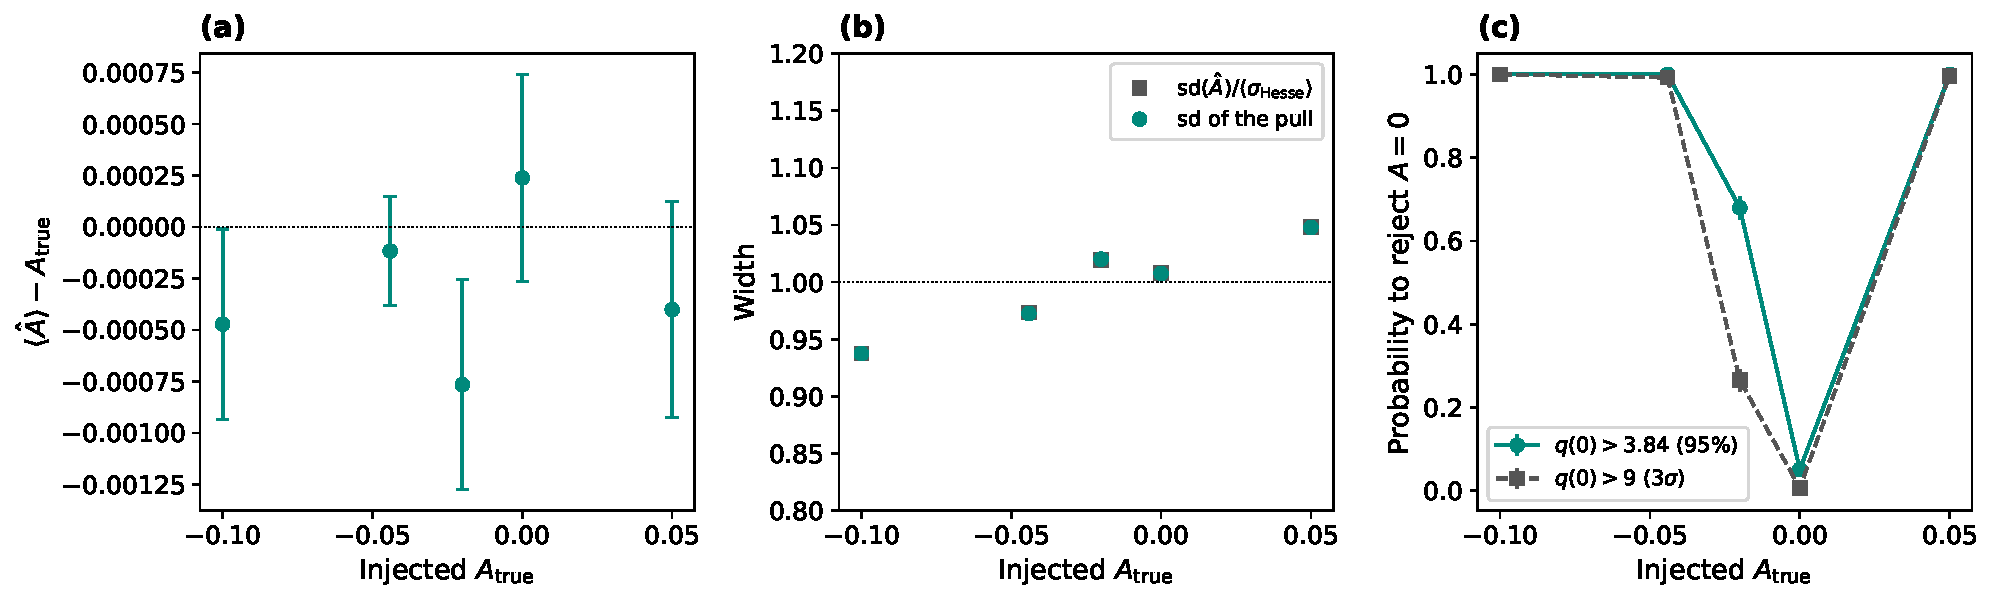
\includegraphics[width=0.75\textwidth]{figures/validation_injection_power.pdf}
\caption{Toy-MC experiments at five injected asymmetries. (a) Bias of $\hat A$, with its standard error. (b) Spread of the estimates divided by the mean Hesse uncertainty, and width of the pulls. (c) Probability to reject $A=0$ in the test with $q(0)>3.84$ (size $5\%$) and $q(0)>9$ ($3\sigma$), as a function of the injected value: size at $A_{\mathrm{true}}=0$, power elsewhere.}
\label{fig:validation_injection}
\end{figure*}

\FloatBarrier
\subsection{Goodness of Fit and the Binning}
\label{sec:validation_gof}
\emph{In short: the binned $\chi^2$ of toy-MC experiments follows its asymptotic distribution, so its $p$-values are accurate; the misfit of the data is $5.4$ standard deviations at $10\,\MeV$ bins and $2.0$ at $2.5\,\MeV$, because it lives on the scale of the flanks of the peak.}
Figure~\ref{fig:validation_gof} compares the binned $\chi^2$ of the toy-MC experiments with its asymptotic distribution and with the data, for the two binnings.
\begin{figure*}[!tbp]
\centering
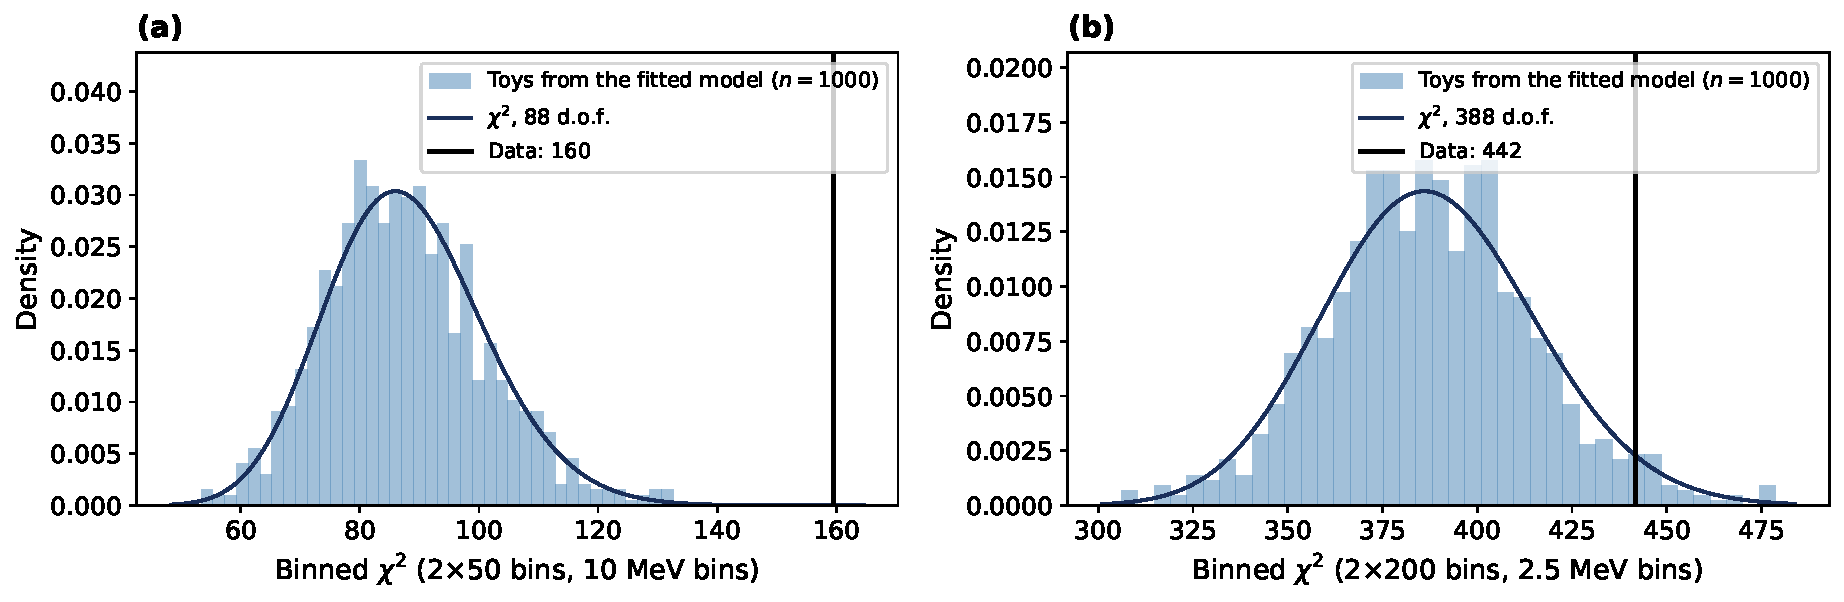
\includegraphics[width=0.75\textwidth]{figures/validation_gof_toys.pdf}
\caption{Binned $\chi^2$ of $1000$ toy-MC experiments from the fitted model, $\chi^2$ distribution with the corresponding degrees of freedom, and value of the data: (a) $2\times50$ bins of $10\,\MeV$, (b) $2\times200$ bins of $2.5\,\MeV$.}
\label{fig:validation_gof}
\end{figure*}

\FloatBarrier
\section{Local Asymmetry in the Dalitz Plane}
\label{app:ext_dalitz}
\emph{In short: the local deviations and their robustness, the null tests of the procedure, the region of the published analysis and the split by magnet polarity.}
\FloatBarrier
\subsection{Local Deviations and Their Robustness}
\emph{In short: two bins have $|S_i|>3$ ($-3.7$ and $-3.0$) and the global homogeneity test gives $\chi^2=80.8$ for $31$ degrees of freedom ($p=3\times10^{-6}$), also in the signal window alone.}

\FloatBarrier
\subsection{Homogeneity Test: Signal Window, Vetoes, Grids and Magnet Split}
\emph{In short: the homogeneity test holds in the signal window, with the charm vetoes and for other grids, and the structure is the same in the two magnet polarities ($\chi^2=23.0$ for $29$ bins).}

\FloatBarrier
\subsection{Null Tests of the Local-Asymmetry Procedure}
\label{sec:dalitz_null}
\emph{In short: permuting the charges gives $\chi^2=31.5\pm8.4$, as expected, and never reaches the observed $80.8$; the phase-space simulation is consistent with no asymmetry, with slightly optimistic $\chi^2$ $p$-values.}

\FloatBarrier
\subsection{Distribution of the Homogeneity Statistic under Charge Permutation}
\label{app:dalitz_perm}
\emph{In short: shuffling the charges reproduces the $\chi^2$ distribution of a uniform asymmetry, and the observed value lies far beyond all $2000$ permutations.}
Figure~\ref{fig:dalitz_perm} shows the distribution of the homogeneity statistic over the permutations against the observed value.
\begin{figure}[!htbp]
\centering
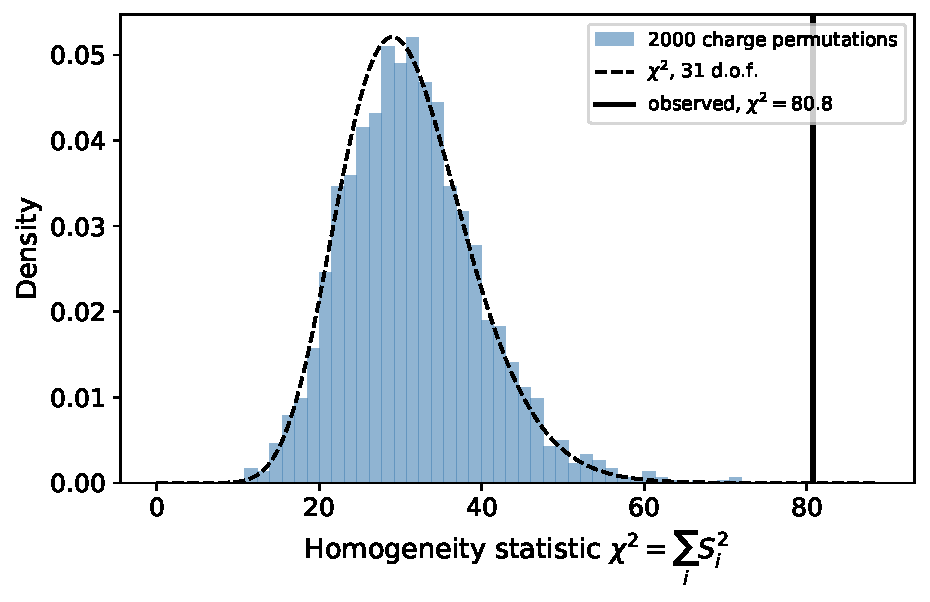
\includegraphics[width=0.4\textwidth]{figures/dalitz_permutation.pdf}
\caption{Homogeneity statistic $\chi^2=\sum_iS_i^2$ of the $8\times8$ Dalitz grid for $2000$ random permutations of the charges (histogram), $\chi^2$ distribution with $31$ degrees of freedom (dashed) and observed value (line).}
\label{fig:dalitz_perm}
\end{figure}

\FloatBarrier
\subsection{Asymmetry in the $\phi(1020)$ Band and in the Significant Bins}
\label{app:dalitz_phi}
\emph{In short: the band of the $\phi(1020)$ has no asymmetry; the negative asymmetry is outside it, and larger when the $\phi$ candidates are removed.}
Figure~\ref{fig:dalitz_phi} shows the distribution of $m_{\mathrm{lo}}$ around the $\phi(1020)$ (a) and the asymmetry of the band and of the significant bins (b).
\begin{figure*}[!tbp]
\centering
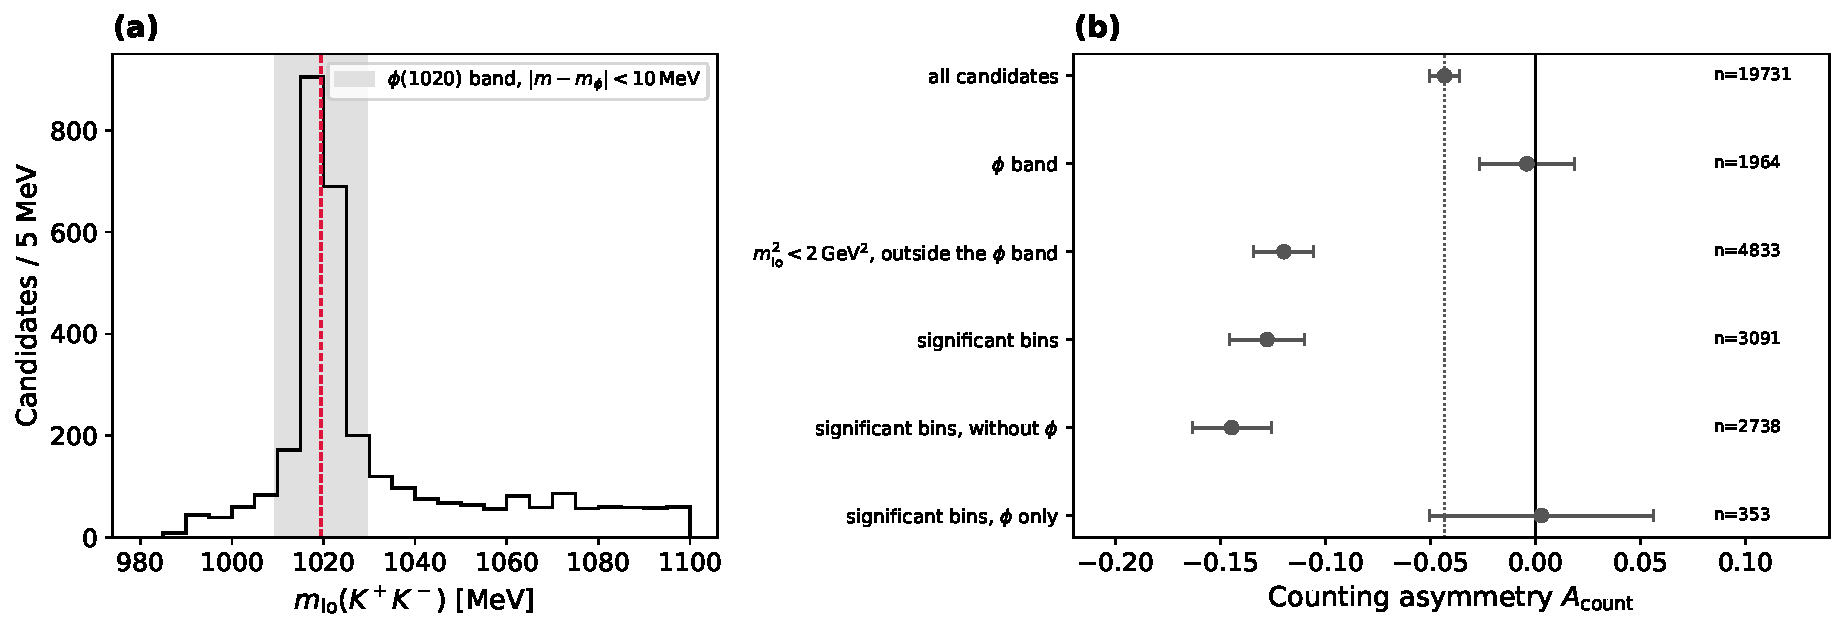
\includegraphics[width=0.75\textwidth]{figures/dalitz_phi_band.pdf}
\caption{(a) Distribution of $m_{\mathrm{lo}}(K^+K^-)$ around the $\phi(1020)$ ($5\,\MeV$ bins) and band used (shaded). (b) Counting asymmetry, with binomial uncertainty and number of candidates, of all candidates (dotted line), of the $\phi$ band, of the region $m^2_{\mathrm{lo}}<2\,\GeV^2$ outside the band, and of the two significant bins of Fig.~\ref{fig:bayes_dalitz}, with and without the candidates of the $\phi$ band, and of those candidates alone.}
\label{fig:dalitz_phi}
\end{figure*}

\FloatBarrier
\subsection{Region of the Published Analysis}
\emph{In short: the $\phi(1020)$ band has no asymmetry ($-0.004\pm0.023$); the fit of the $2146$ candidates of the published region gives $-0.234\pm0.025$ (Bayesian) and $-0.237\pm0.025$ (frequentist), against $-0.239\pm0.020$.}

\FloatBarrier
\section{Comparison of the Two Approaches}
\label{app:ext_comp}
\emph{In short: the numerical agreement of the two fits, the meaning of the intervals, the hypothesis tests, the profile likelihood against the posterior, and the two methods at low statistics.}
\FloatBarrier
\subsection{Numerical Agreement}
\label{sec:comparison_numbers}
\emph{In short: the two fits agree to the quoted digits (estimates differ by $0.0002$, both uncertainties are $0.0085$, systematic uncertainties $0.0070$ and $0.0072$); sideband subtraction gives $-0.0503\pm0.0083$.}

\FloatBarrier
\subsection{Meaning of the Interval}
\emph{In short: the credible interval is a probability on $A$ given the data and the prior, the confidence interval a property of the procedure, which the bootstrap and the toy experiments verified.}

\FloatBarrier
\subsection{Profile Likelihood, Posterior and the Two Polarities}
\label{sec:checks_profile}
\emph{In short: profiling and marginalizing the nuisance parameters give the same distribution of $A$; the two magnet polarities agree with each other, and combining their likelihoods reproduces the joint fit.}
Table~\ref{tab:checks_polarity} gives $\Araw$ for the two magnet polarities and for their combination, by the two methods.
\begin{table}[!htbp]
\centering
\resizebox{\ifdim\width>\linewidth\linewidth\else\width\fi}{!}{\begin{tabular}{lcc}
\toprule
 & Frequentist & Bayesian \\
\midrule
Magnet down & $-0.0492\pm0.0111$ & $-0.0497\pm0.0112$ \\
Magnet up & $-0.0374\pm0.0131$ & $-0.0378\pm0.0129$ \\
Combination of the two & $-0.0443\pm0.0084$ & $-0.0446\pm0.0086$ \\
Joint fit & $-0.0441\pm0.0085$ & $-0.0443\pm0.0085$ \\
\bottomrule
\end{tabular}}
\caption{$\Araw$ for the two magnet polarities and their combination, by the two methods; the frequentist combination is the sum of the profile likelihoods of the two polarities, the Bayesian one the sequential update of the posterior.}
\label{tab:checks_polarity}
\end{table}

\FloatBarrier
\subsection{Confidence and Credible Regions in $(A,A_b)$}
\label{sec:checks_region}
\emph{In short: the $68\%$ and $95\%$ regions of the frequentist profile ($\Delta\mathrm{NLL}$ at the $\chi^2_2$ values $2.30$ and $5.99$) and of the Bayesian highest posterior density coincide, and $A=0$ lies outside both.}
Figure~\ref{fig:checks_region} shows the frequentist and the Bayesian regions in the $(A,A_b)$ plane.
\begin{figure}[!htbp]
\centering
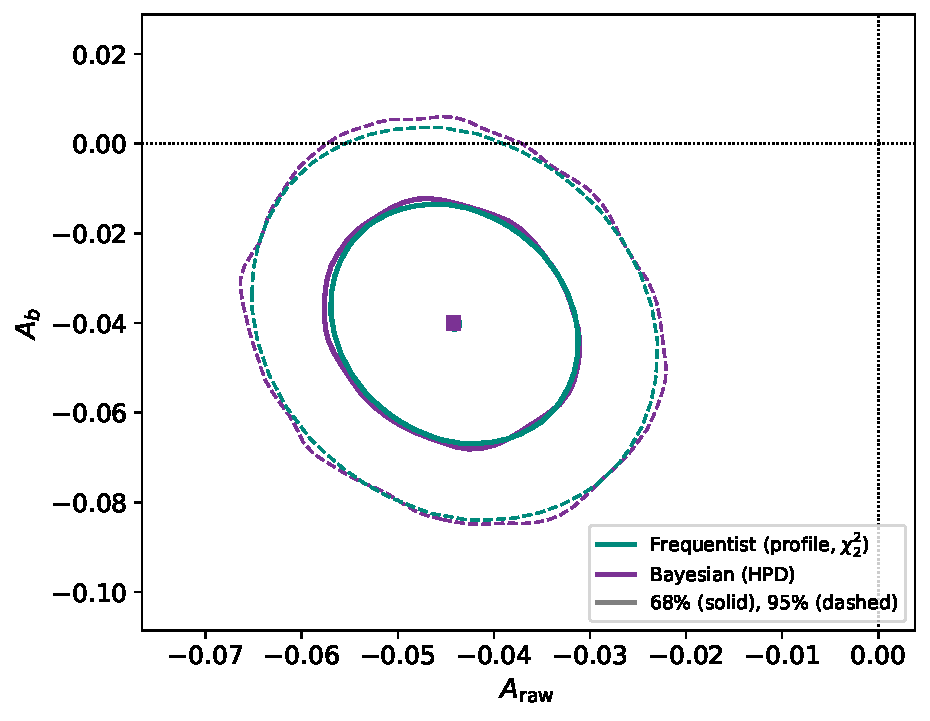
\includegraphics[width=0.4\textwidth]{figures/validation_region_Ab.pdf}
\caption{$68\%$ (solid) and $95\%$ (dashed) regions in $(A,A_b)$: frequentist, from the profile likelihood with $\chi^2_2$ thresholds, and Bayesian, highest-posterior-density regions of the chain. Dots: best-fit and posterior median.}
\label{fig:checks_region}
\end{figure}

\FloatBarrier
\subsection{Hypothesis Test}
\emph{In short: the exact binomial test on all candidates gives $6.1\sigma$, the test of the fit $p=2\times10^{-7}$ ($5.2\sigma$) and the Bayes factor $BF_{10}\approx9\times10^3$; they answer different questions.}

\FloatBarrier
\subsection{Goodness of Fit}
\emph{In short: the same fit has $p=0.03$ in $2.5\,\MeV$ bins and $p\approx5\times10^{-6}$ in $10\,\MeV$ bins: the $p$-value of the binned $\chi^2$ is a property of the binning as much as of the model.}

\FloatBarrier
\subsection{Nuisance Parameters and Validation}
\emph{In short: the frequentist analysis profiles the eleven nuisance parameters and the Bayesian one marginalizes them; the results coincide because $A$ is almost uncorrelated with them.}

\FloatBarrier
\subsection{Published Analysis: Samples and Models}
\emph{In short: the published analysis has $22{,}119\pm164$ signal candidates, a Cruijff signal and misidentified and partially reconstructed backgrounds; with the same $D^0$ veto the Bayesian fit gives $-0.0496\pm0.0088$.}

\FloatBarrier
\subsection{Published Analysis: Raw versus CP Asymmetry}
\emph{In short: $\ACP\approx\Araw-A_P-A_D$; the corrections move the published result from $-0.060$ to $-0.043\pm0.009\pm0.003\pm0.007$ and cannot be assumed for a different selection.}

\FloatBarrier
\subsection{Machine-Learning Cross-Check}
\emph{In short: a cut at $0.5$ on the classifier score keeps $92\%$ of the signal and $36\%$ of the background and gives $-0.0451\pm0.0087$ (Bayesian) and $-0.0447\pm0.0086$ (frequentist).}

\FloatBarrier
\subsection{Bayesian and Frequentist Intervals at Low Statistics}
\label{sec:bayes_lowstat}
\emph{In short: credible and confidence intervals coincide for $\sim2\times10^4$ candidates with flat priors, and stay equal, in value and coverage, down to $50$ candidates.}
Figure~\ref{fig:bayes_lowstat} shows the coverage of the credible, Minos and Hesse intervals against the number of candidates.
\begin{figure*}[!tbp]
\centering
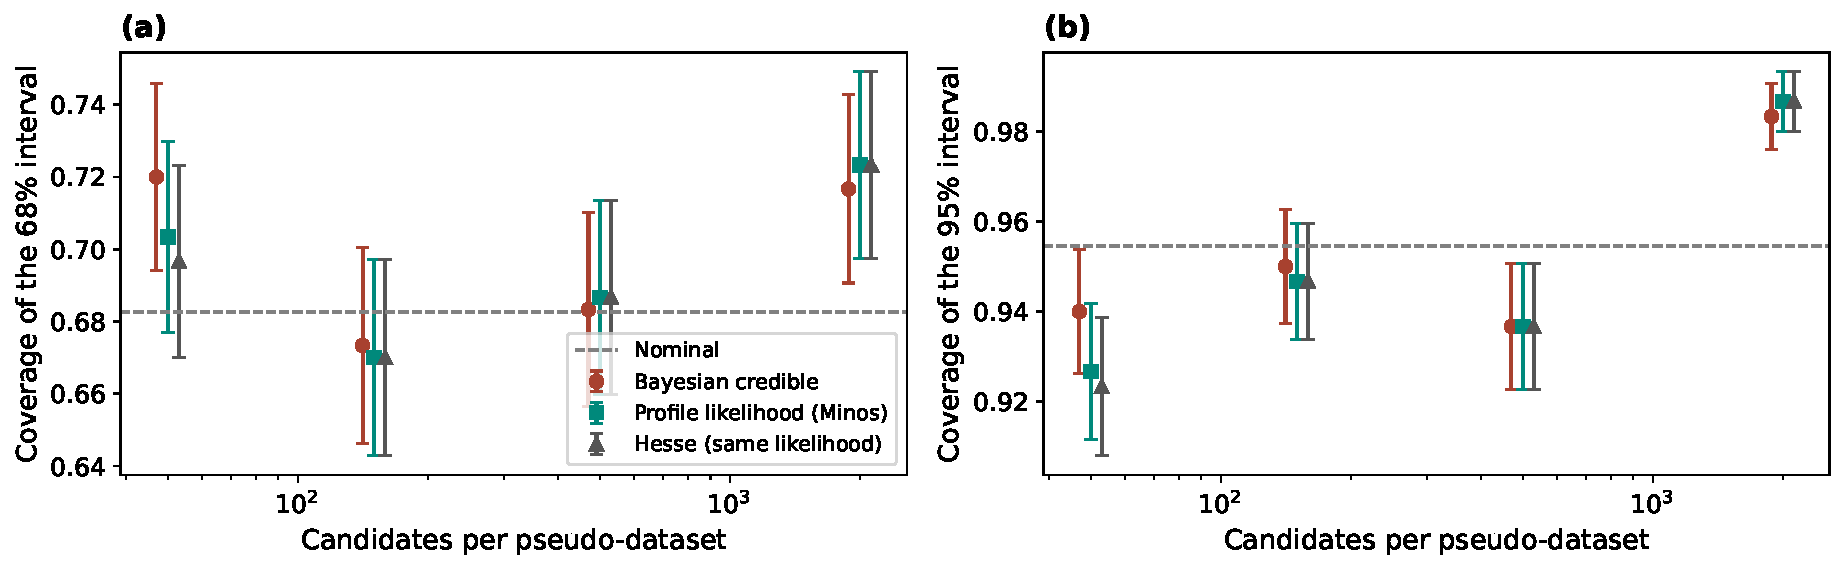
\includegraphics[width=0.75\textwidth]{figures/bayes_nominal_lowstat.pdf}
\caption{Coverage of the (a) 68\% and (b) 95\% intervals on $A$ vs the number of candidates, for the Bayesian credible interval, the profile-likelihood (Minos) interval and the Hesse interval of the same likelihood; 300 toy-MC datasets per point, binomial uncertainties. The dashed lines mark the nominal coverage ($1\sigma$, $2\sigma$; the Bayesian 95\% interval is the 2.5--97.5\% one).}
\label{fig:bayes_lowstat}
\end{figure*}

\FloatBarrier
\section{Machine-Learning Analysis}
\label{sec:ml}
\emph{In short: classifiers trained on weak labels from the mass spectrum (there are no true labels) reach a test AUC of $0.86$; a cut on their score leaves $\Araw$ unchanged, and an adaptive partition of the Dalitz plane shows the same pattern as the fixed binning.}
\FloatBarrier
\subsection{Background: Regularization, Bias-Variance and Loss Functions}
\label{app:theory_ml}
\emph{In short: cross-entropy is a Bernoulli negative log-likelihood, $L1$ and $L2$ penalties shrink the coefficients, the test error splits into bias, variance and noise, and class weights rescale the score by a known factor.}

\FloatBarrier
\subsection{Background: Classification Without Labels}
\emph{In short: the classifier that is optimal between two mixtures of the same signal and background is monotonic in the signal-to-background ratio, so labels derived from the mass are sufficient.}

\FloatBarrier
\subsection{Background: Clustering and Uncertainty Estimators}
\emph{In short: $K$-means converges to a local minimum of the inertia, the adjusted Rand index measures the stability of a partition, and the spread of an ensemble estimates the epistemic uncertainty.}

\FloatBarrier
\subsection{Weak Labels and Feature Set}
\label{sec:ml_labels}
\emph{In short: a classifier separates a signal-enriched window from the mass sidebands ($15{,}130$ signal-like and $1940$ background-like candidates, $20$ features, $60/20/20$ split); by the Neyman-Pearson argument of the CWoLa approach it is also the signal/background classifier, if the features carry no information on the mass.}
Figure~\ref{fig:ml_labels} shows the signal-like and background-like candidates on the mass spectrum.
\begin{figure}[!htbp]
\centering
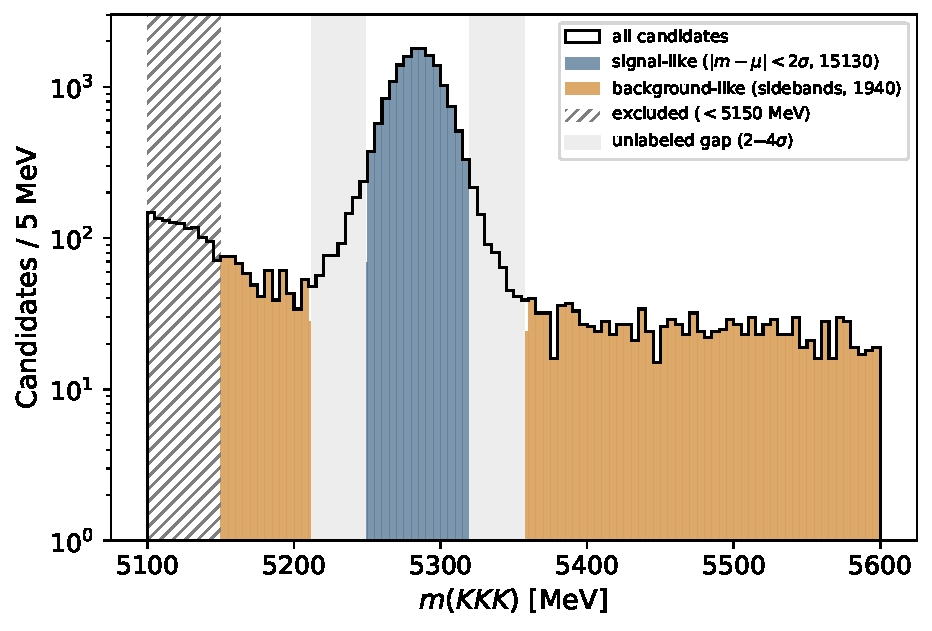
\includegraphics[width=0.4\textwidth]{figures/ml_weak_labels.pdf}
\caption{Weak labels on the mass spectrum of the fit window: signal-like candidates ($|m-\mu|<2\sigma$, $15{,}130$) and background-like candidates (sidebands beyond $4\sigma$ and above $5150\,\MeV$, $1940$); the $2$--$4\sigma$ gap is left unlabeled and the region below $5150\,\MeV$, where the background rises towards partially reconstructed decays, is excluded.}
\label{fig:ml_labels}
\end{figure}

\FloatBarrier
\subsection{Model Comparison}
\label{sec:ml_models}
\emph{In short: six classifiers; the tree ensembles and the neural network reach test AUC $0.857$--$0.864$, about $0.09$ above the linear models and indistinguishable from each other within the test-set uncertainty ($0.012$); gradient boosting, best in cross-validation, is the reference.}
Table~\ref{tab:ml_models} gives the cross-validated and test AUC and the Brier score of each model, Fig.~\ref{fig:ml_roc} the ROC curves and Fig.~\ref{fig:ml_features} the feature importance.
\begin{table}[!htbp]
\centering
\begin{tabular}{lccc}
\toprule
Model & CV AUC & Test AUC & Brier \\
\midrule
Logistic Regression       & $0.769 \pm 0.016$ & $0.771 \pm 0.013$ & $0.197$ \\
Logistic Regression (L1)  & --                & $0.771 \pm 0.013$ & $0.198$ \\
Decision Tree             & $0.816 \pm 0.011$ & $0.824 \pm 0.013$ & $0.133$ \\
Random Forest             & $0.863 \pm 0.017$ & $0.860 \pm 0.012$ & $0.122$ \\
Gradient Boosting         & $\mathbf{0.866 \pm 0.016}$ & $0.864 \pm 0.012$ & $0.116$ \\
FFNN                      & --                & $0.857 \pm 0.012$ & $0.134$ \\
\bottomrule
\end{tabular}
\caption{Cross-validated AUC (mean and standard deviation over the folds), test-set AUC (with bootstrap uncertainty) and test-set Brier score of the raw scores. Gradient boosting, best in cross-validation, is the reference model. The FFNN is validated on the validation set instead of by cross-validation.}
\label{tab:ml_models}
\end{table}
\begin{figure}[!htbp]
\centering
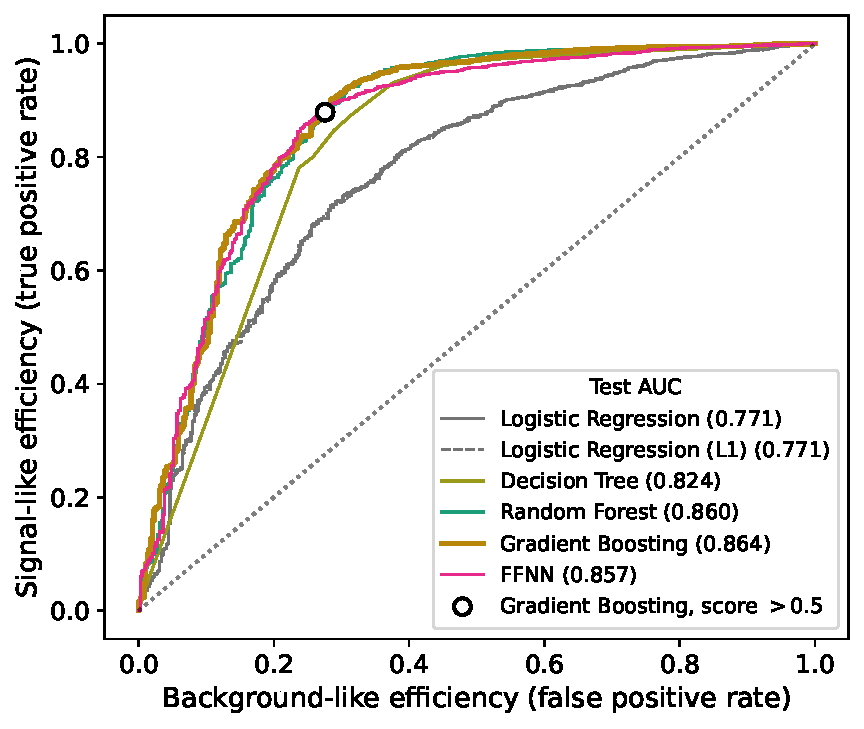
\includegraphics[width=0.4\textwidth]{figures/ml_nominal_roc.pdf}
\caption{ROC curves on the test set, with the test AUC of each model in the legend (Table~\ref{tab:ml_models}); the reference model is drawn thicker, and the two logistic regressions overlap. The circle marks the cut on the reference score used in Appendix~\ref{sec:ml_stability}.}
\label{fig:ml_roc}
\end{figure}
\begin{figure*}[!tbp]
\centering
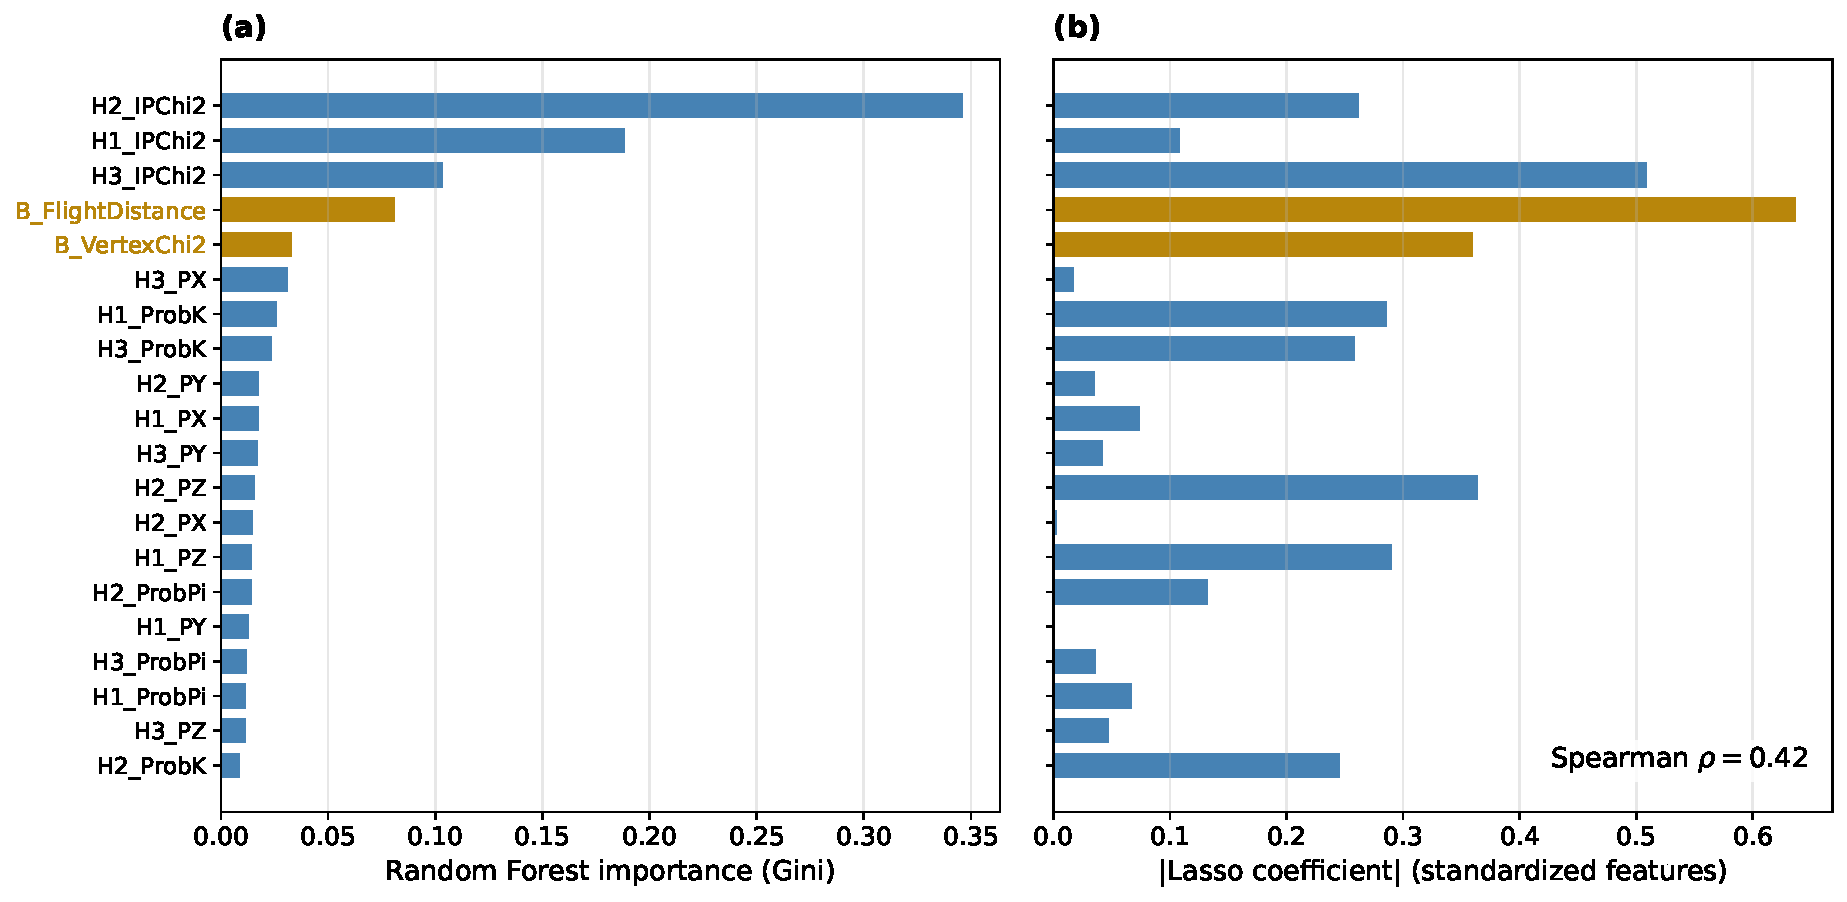
\includegraphics[width=0.75\textwidth]{figures/ml_nominal_features.pdf}
\caption{Random Forest feature importance (Gini, a) and magnitude of the Lasso coefficient of the standardized feature (b) for the 20 features, both ordered by Random Forest importance; the two $B$-candidate variables are highlighted.}
\label{fig:ml_features}
\end{figure*}

\FloatBarrier
\subsection{Regularization, Bias-Variance, and Calibration}
\label{sec:ml_regcal}
\emph{In short: the linear model does not overfit, gradient boosting overfits beyond $\sim$150 stages without losing test AUC, and class weights bias the probabilities, which an isotonic recalibration corrects (Brier score $0.122\to0.062$) without changing the ranking.}
Figure~\ref{fig:ml_regularization} shows the cross-validated AUC against the regularization strength, Fig.~\ref{fig:ml_bias_variance} the accuracy and the AUC of gradient boosting against the number of stages, and Fig.~\ref{fig:ml_calibration} the reliability diagram of the Random Forest.
\begin{figure}[!htbp]
\centering
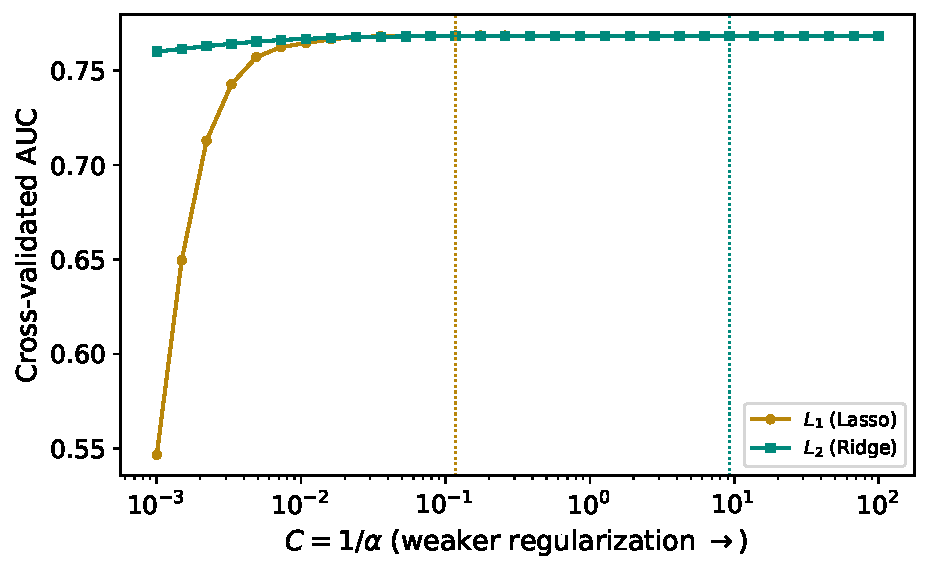
\includegraphics[width=0.4\textwidth]{figures/ml_regularization.pdf}
\caption{Cross-validated AUC of the logistic regression against the inverse regularization strength $C=1/\alpha$ ($30$ log-spaced values), for the $L_1$ (Lasso) and $L_2$ (Ridge) penalties; the dotted lines mark the optimum of each.}
\label{fig:ml_regularization}
\end{figure}
\begin{figure*}[!tbp]
\centering
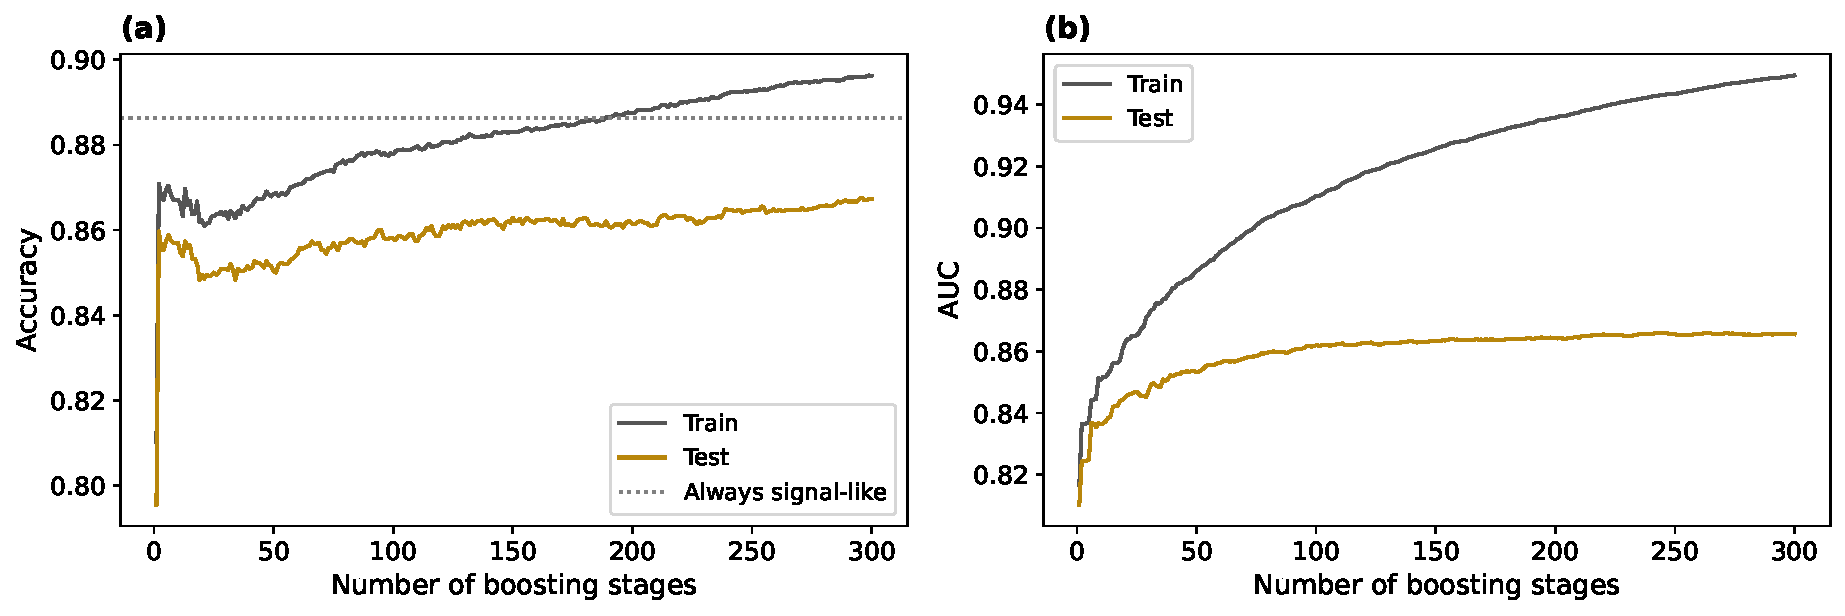
\includegraphics[width=0.75\textwidth]{figures/ml_nominal_bias_variance.pdf}
\caption{Gradient boosting: (a) accuracy at the $0.5$ threshold and (b) AUC on the training and test sets as a function of the number of boosting stages. The dotted line is the accuracy of always predicting the signal-like class.}
\label{fig:ml_bias_variance}
\end{figure*}
\begin{figure}[!htbp]
\centering
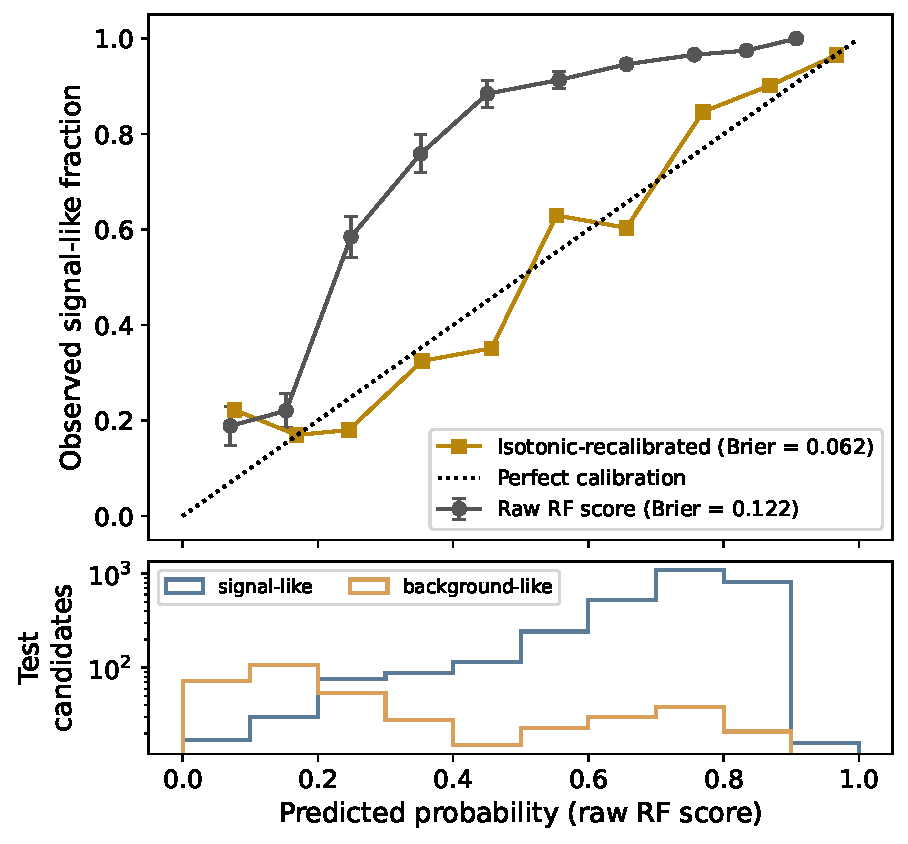
\includegraphics[width=0.4\textwidth]{figures/ml_nominal_calibration.pdf}
\caption{Reliability diagram of the Random Forest on the test set: observed fraction of signal-like candidates vs.\ predicted probability, for the raw score (with binomial uncertainties) and for the isotonic-recalibrated one. Bottom: distribution of the raw score for the two weak-label classes; the low-probability bins contain few candidates.}
\label{fig:ml_calibration}
\end{figure}

\FloatBarrier
\subsection{Uncertainty Quantification}
\label{sec:ml_uncertainty}
\emph{In short: the three estimators give mean per-candidate uncertainties of $0.178$ (Random Forest), $0.095$ (MC dropout) and $0.050$ (deep ensemble); they measure different sources of variability, and only the Random Forest spread visibly decreases with the training-set size.}
Figure~\ref{fig:ml_uncertainty} shows the three estimators of the per-candidate uncertainty and the dependence of the Random Forest spread on the size of the training set.
\begin{figure*}[!tbp]
\centering
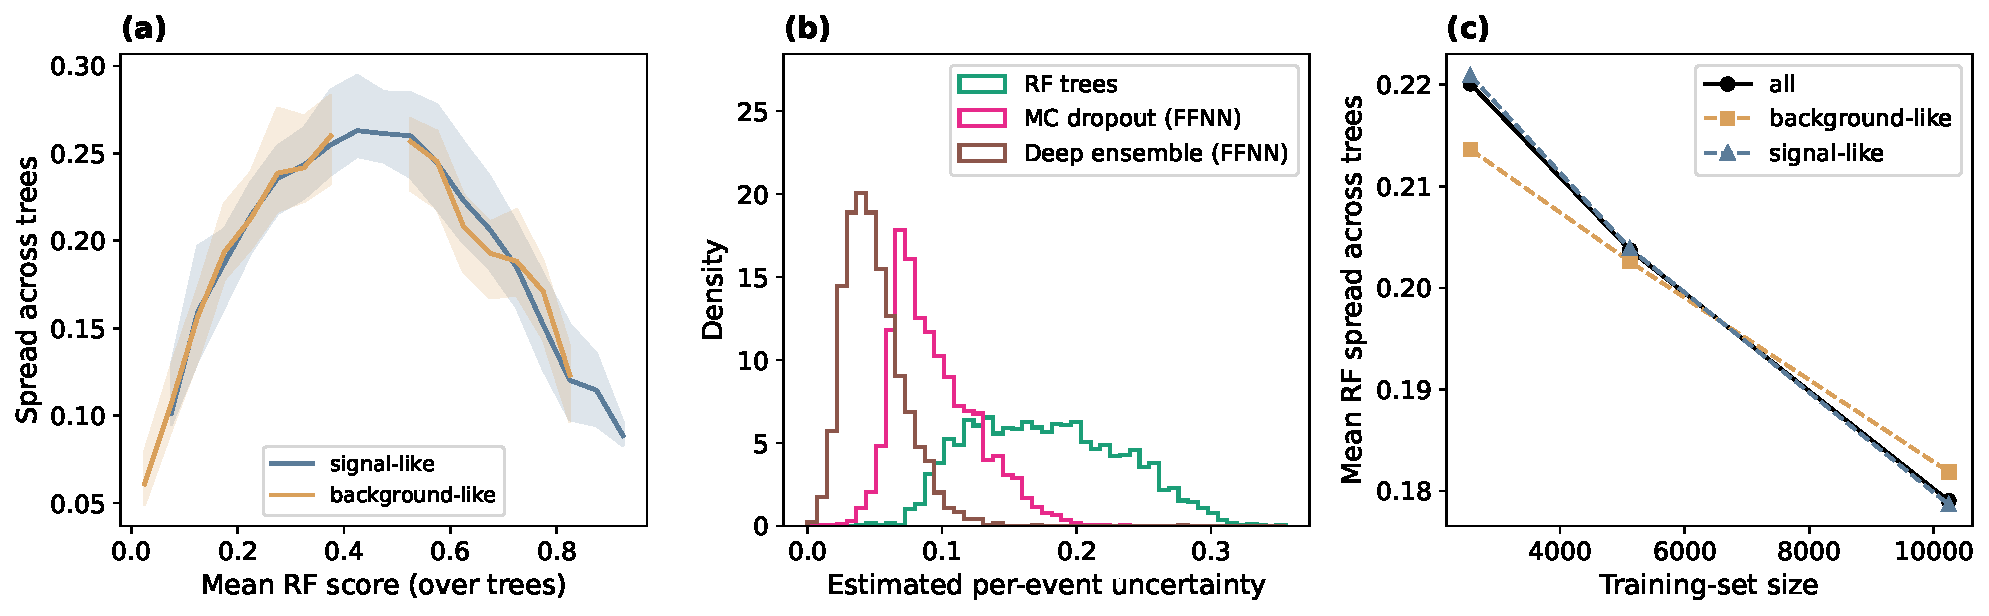
\includegraphics[width=0.75\textwidth]{figures/ml_nominal_uncertainty.pdf}
\caption{(a) Spread across the Random Forest trees vs.\ mean tree score, median and 16--84\% band of the test candidates of each weak-label class. (b) Distributions of the per-candidate uncertainty from the Random Forest trees, MC dropout and the deep ensemble. (c) Mean Random Forest spread vs.\ training-set size, for all, background-like and signal-like test candidates.}
\label{fig:ml_uncertainty}
\end{figure*}

\FloatBarrier
\subsection{K-means on the Dalitz Plot}
\label{sec:ml_kmeans}
\emph{In short: for $K=8$ two clusters deviate by more than $3\sigma$ ($\chi^2=46.4$ for $7$ degrees of freedom): a negative asymmetry at low $m^2_{\mathrm{lo}}$ and positive ones at high $m^2_{\mathrm{hi}}$, as in the fixed binning.}
Figure~\ref{fig:ml_kmeans_sel} shows the inertia and the silhouette against $K$, and Fig.~\ref{fig:ml_kmeans} the partition with $K=8$ coloured by the significance of each cluster.
\begin{figure*}[!tbp]
\centering
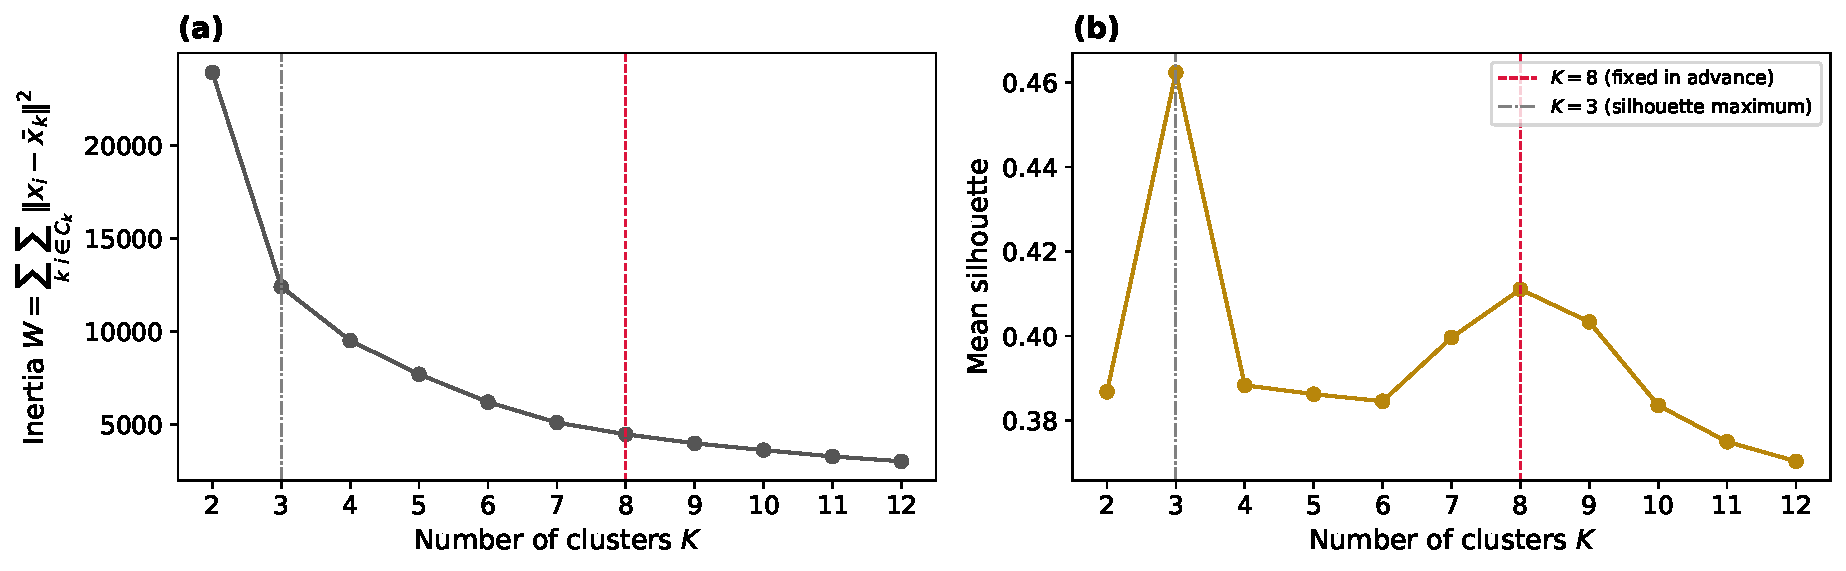
\includegraphics[width=0.85\textwidth]{figures/ml_kmeans_selection.pdf}
\caption{(a) Inertia and (b) mean silhouette of the $K$-means partition of the Dalitz plane for $K=2$--$12$; the dashed line marks the $K=8$ fixed in advance and the dash-dotted line the maximum of the silhouette, $K=3$.}
\label{fig:ml_kmeans_sel}
\end{figure*}
\begin{figure}[!htbp]
\centering
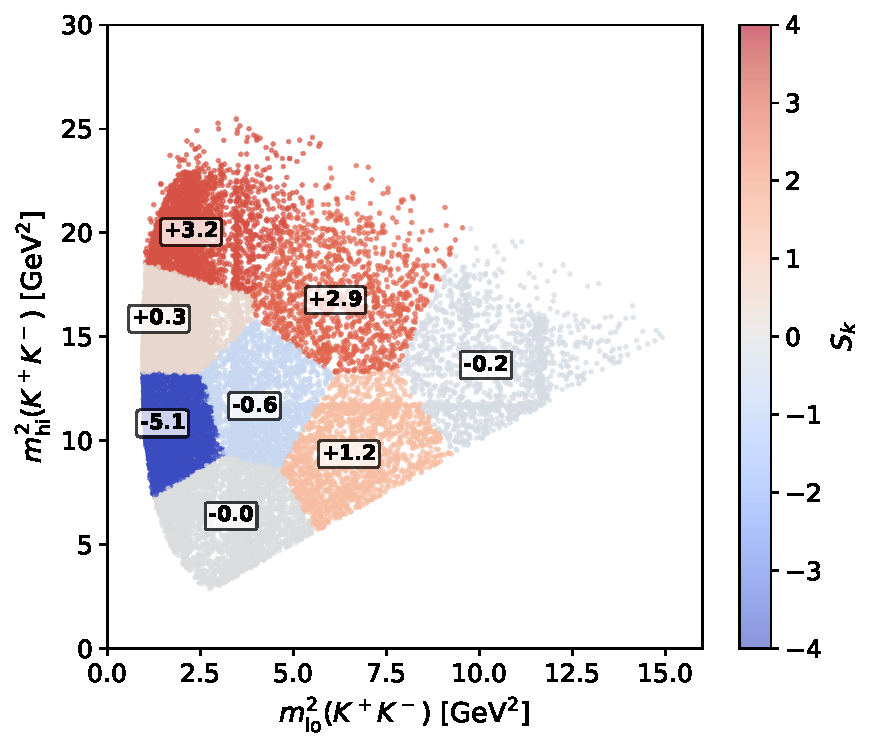
\includegraphics[width=0.4\textwidth]{figures/ml_nominal_kmeans.pdf}
\caption{$K$-means partition ($K=8$) of the Dalitz plane, all candidates of the fit window, same axes as Fig.~\ref{fig:bayes_dalitz}. Color and labels: local significance of each cluster with respect to the global asymmetry, $S_k=(A_k-A_{\mathrm{glob}})/\sigma(A_k)$, on the same scale as panel (c) of Fig.~\ref{fig:bayes_dalitz}.}
\label{fig:ml_kmeans}
\end{figure}

\FloatBarrier
\subsection{Stability of $\Araw$ under ML Selection}
\label{sec:ml_stability}
\emph{In short: a cut on the score at $0.5$ keeps $92\%$ of the signal and $36\%$ of the background and leaves $\Araw$ within its expected statistical spread with both fits and with counting; it does not improve the precision and cannot remove the misidentified background.}
Figure~\ref{fig:ml_threshold} shows the counting asymmetry against the score threshold; Table~\ref{tab:three_methods} and Fig.~\ref{fig:ml_three} compare the three methods on the full and on the selected sample; Fig.~\ref{fig:ml_mass_cut} shows the mass spectrum before and after the cut and the efficiency of the cut, and Fig.~\ref{fig:ml_high_bkg} the high-background sample.
\begin{figure}[!htbp]
\centering
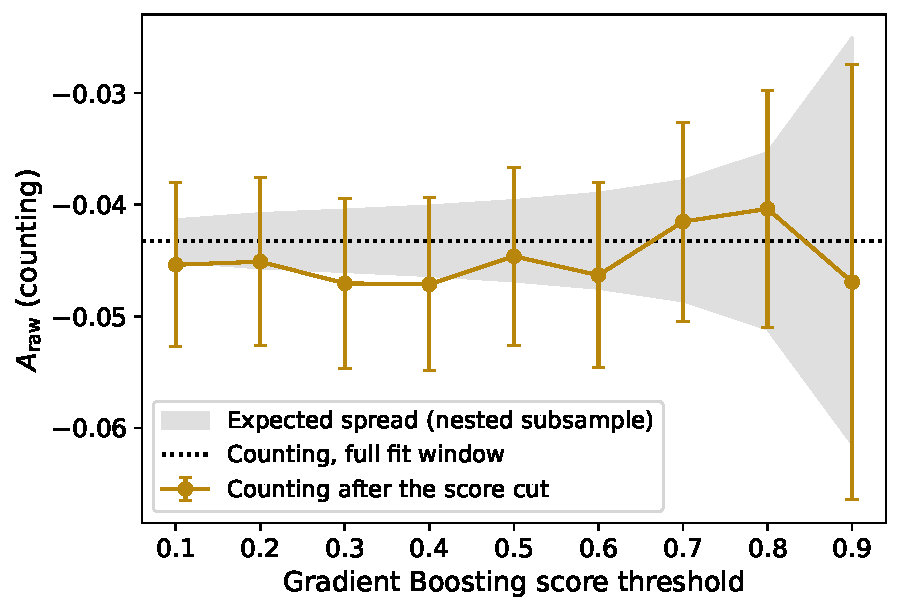
\includegraphics[width=0.4\textwidth]{figures/ml_nominal_threshold.pdf}
\caption{Counting asymmetry after a cut on the gradient-boosting score, vs.\ threshold, with its binomial uncertainty. Dotted line: counting asymmetry of the full fit window; band: expected statistical spread of a nested subsample around it, $\pm\sqrt{\sigma_{\mathrm{sub}}^2-\sigma_{\mathrm{full}}^2}$.}
\label{fig:ml_threshold}
\end{figure}
\begin{table*}[!tbp]
\centering
\begin{tabular}{lccc}
\toprule
Method & Full sample & Score $>0.5$ & Shift (expected) \\
\midrule
Bayesian fit    & $-0.0443\pm0.0085$ & $-0.0451\pm0.0087$ & $-0.0008\,(0.0018)$ \\
Frequentist fit & $-0.0441\pm0.0085$ & $-0.0447\pm0.0086$ & $-0.0006\,(0.0012)$ \\
Counting        & $-0.0432\pm0.0071$ & $-0.0446\pm0.0080$ & $-0.0014\,(0.0036)$ \\
\bottomrule
\end{tabular}
\caption{$\Araw$ on the full fit window ($19{,}731$ candidates) and after the cut on the gradient-boosting score ($15{,}709$), by the three methods. The expected shift is the statistical spread of a nested subsample, $\sqrt{\sigma_{\mathrm{sub}}^2-\sigma_{\mathrm{full}}^2}$. Counting includes the background.}
\label{tab:three_methods}
\end{table*}
\begin{figure}[!htbp]
\centering
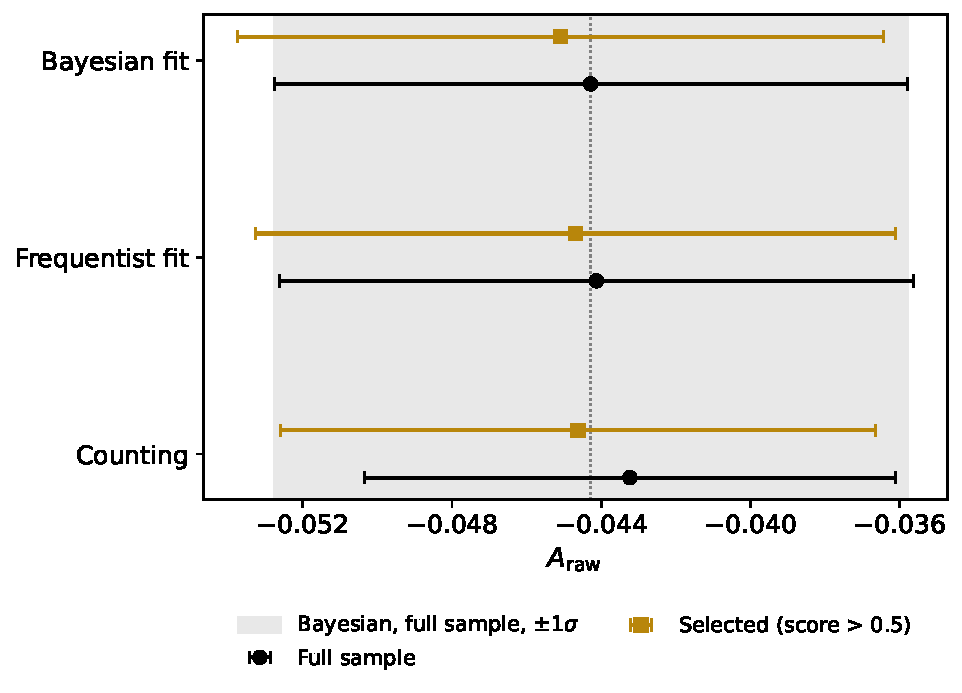
\includegraphics[width=0.4\textwidth]{figures/ml_nominal_three_methods.pdf}
\caption{$\Araw$ from the Bayesian fit, the frequentist fit and counting, for the full sample and the ML-selected one (Table~\ref{tab:three_methods}).}
\label{fig:ml_three}
\end{figure}
\begin{figure*}[!tbp]
\centering
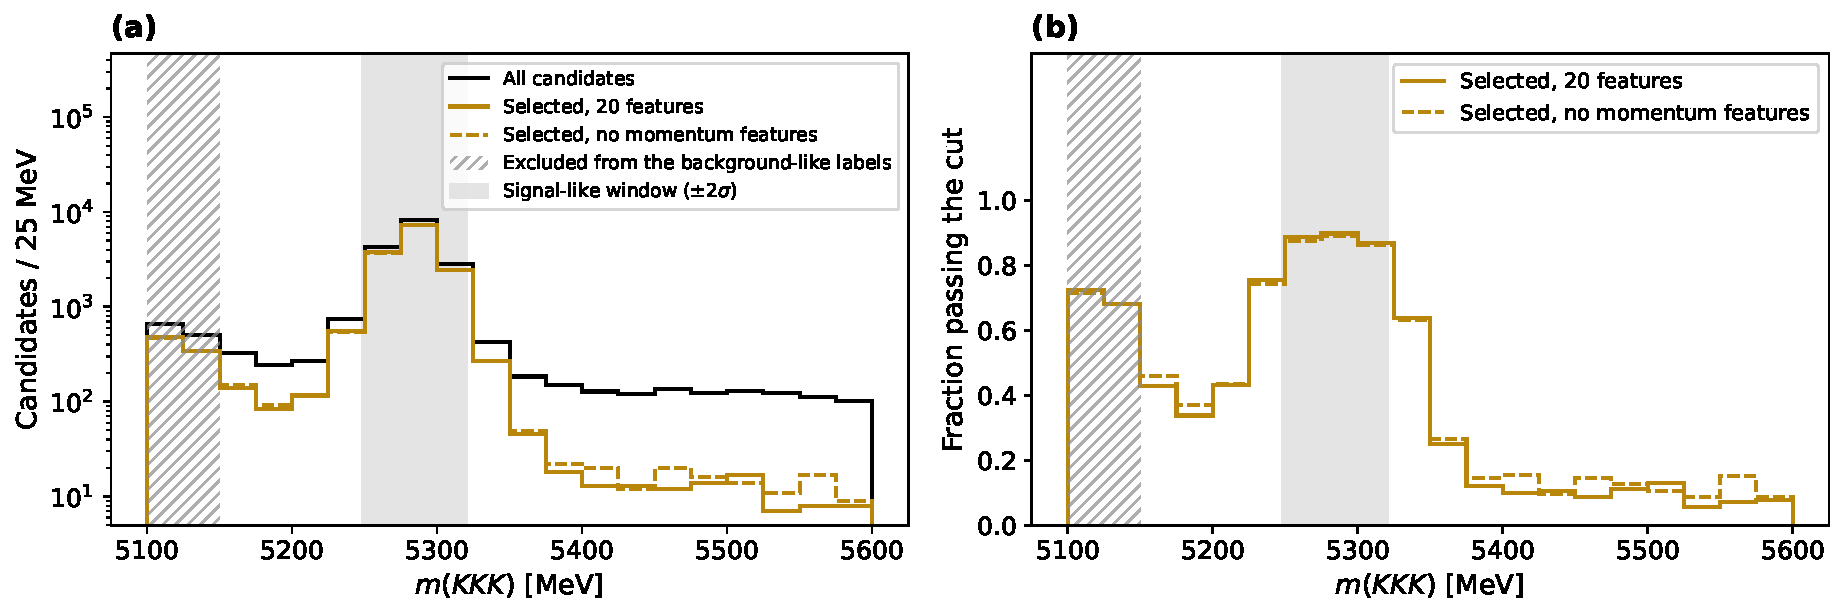
\includegraphics[width=0.75\textwidth]{figures/ml_nominal_mass_after_cut.pdf}
\caption{(a) Mass spectrum of all candidates and of those with gradient-boosting score $>0.5$, for the 20-feature classifier and for one trained without the kaon momentum components (25\,MeV bins). (b) Fraction of candidates passing the cut. Hatched: the region below $5150\,\MeV$ excluded from the background-like labels; grey: the signal-like window.}
\label{fig:ml_mass_cut}
\end{figure*}
\begin{figure*}[!tbp]
\centering
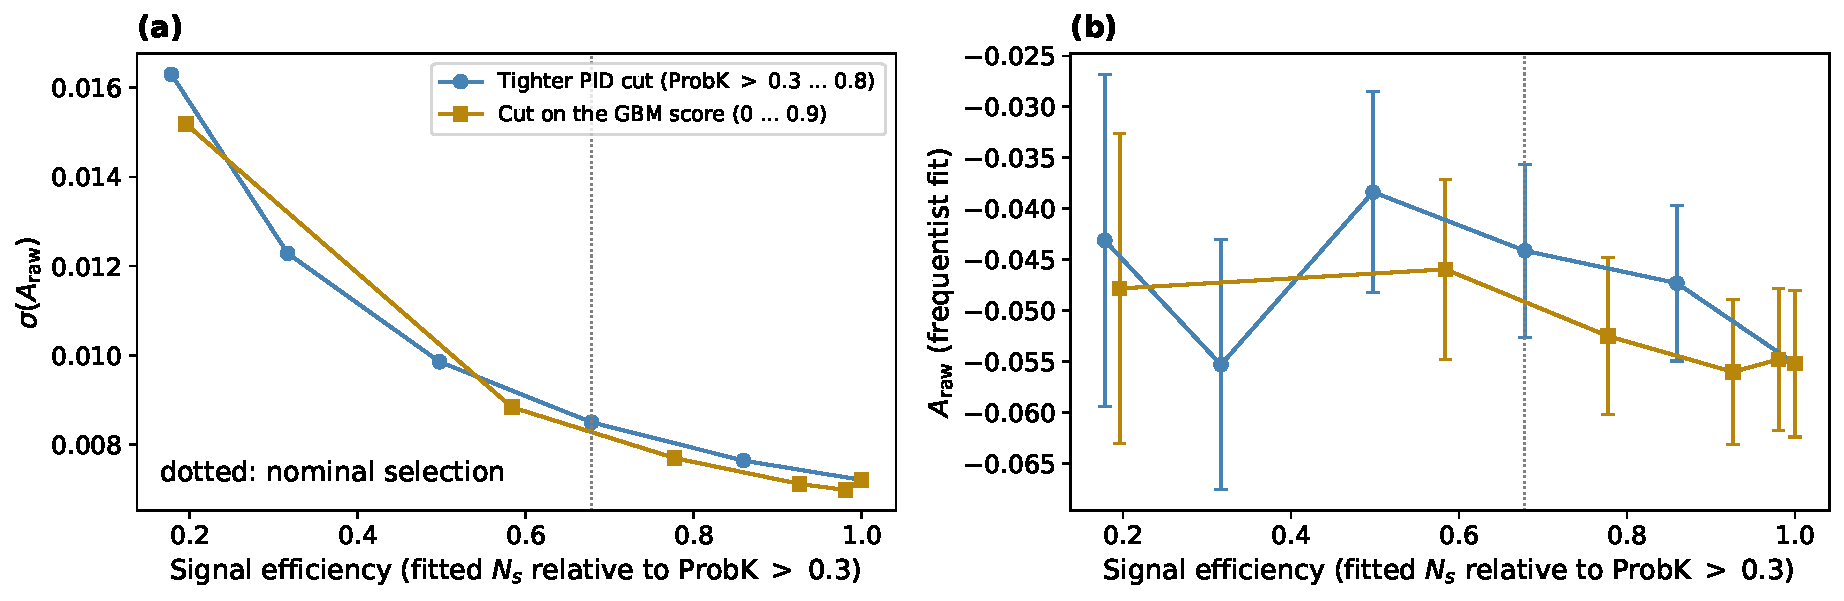
\includegraphics[width=0.75\textwidth]{figures/ml_nominal_high_background.pdf}
\caption{High-background sample ($\texttt{ProbK}>0.3$): (a) statistical uncertainty and (b) value of $\Araw$ from the frequentist fit vs signal efficiency, for tighter identification cuts ($\texttt{ProbK}>0.3,\dots,0.8$) and for cuts on the score of the classifier retrained on this sample ($0,\dots,0.9$). The dotted line marks the nominal selection ($\texttt{ProbK}>0.5$). The samples are nested, so their uncertainties are correlated.}
\label{fig:ml_high_bkg}
\end{figure*}

\FloatBarrier
\subsection{Hyperparameter Optimization}
\label{sec:ml_hyper}
\emph{In short: the best configurations improve the test AUC by at most $0.005$, less than its uncertainty, and the cross-validated maximum overestimates the test AUC (winner's curse).}
Table~\ref{tab:ml_hyperparams} gives the search for the tree ensembles, Fig.~\ref{fig:ml_ffnn_search} the cross-validated AUC of the $168$ FFNN configurations and Table~\ref{tab:ml_ffnn_search} the five best.
\begin{figure}[!htbp]
\centering
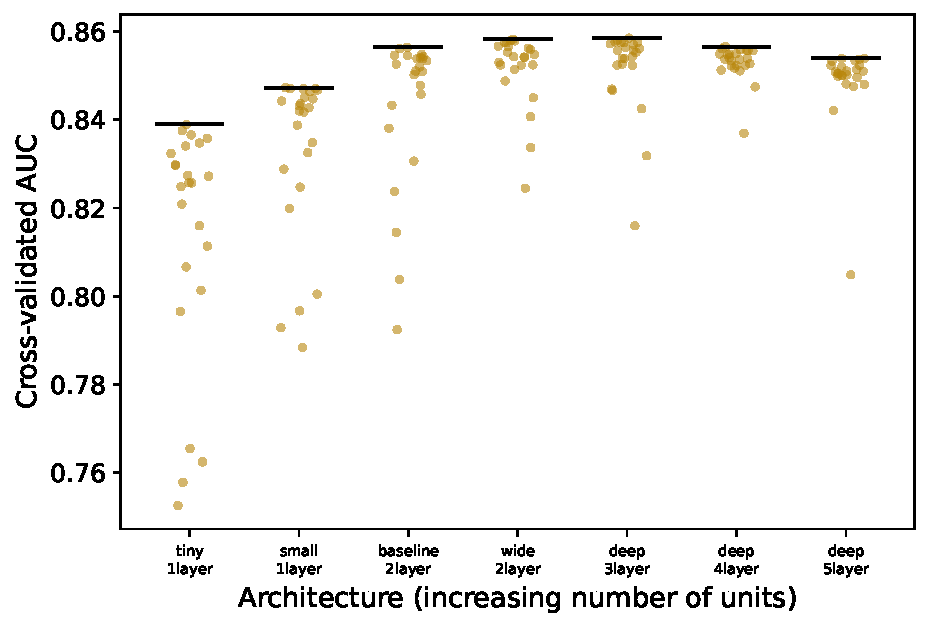
\includegraphics[width=0.4\textwidth]{figures/ml_ffnn_search.pdf}
\caption{Cross-validated AUC of the $168$ FFNN configurations (dots) for each of the seven architectures, ordered by number of units; the black segment marks the best configuration of each architecture.}
\label{fig:ml_ffnn_search}
\end{figure}
\begin{table*}[!tbp]
\centering
\begin{tabular}{lllc}
\toprule
Model & \pcell{7cm}{Grid} & Best configuration & CV AUC / Test AUC (default) \\
\midrule
Random Forest & \pcell{7cm}{\texttt{n\_estimators} $200$--$1200$, \texttt{max\_depth} $6$--$12$ or none, \texttt{min\_samples\_leaf} $5$--$40$} & $400$, $12$, $5$ & $0.8706$ / $0.8656$ ($0.8604$) \\
Gradient Boosting & \pcell{7cm}{\texttt{n\_estimators} $100$--$500$, \texttt{max\_depth} $1$--$5$, \texttt{learning\_rate} $0.01$--$0.1$} & $300$, $2$, $0.1$ & $0.8684$ / $0.8650$ ($0.8643$) \\
\bottomrule
\end{tabular}
\caption{Hyperparameter search for the tree ensembles ($120$ and $100$ configurations, 5-fold cross-validation repeated 10 times, balanced class weights). The test AUC of the best configuration is compared with that of the default of Table~\ref{tab:ml_models} (in parentheses); the bootstrap uncertainty of each test AUC is $0.012$.}
\label{tab:ml_hyperparams}
\end{table*}
\begin{table*}[!tbp]
\centering
\begin{tabular}{llccc}
\toprule
Architecture & Layers & Dropout & Learning rate & CV AUC \\
\midrule
\texttt{deep\_3layer} (best) & $[64,32,16]$ & $0.2$ & $0.003$ & $0.8585\pm0.0174$ \\
\texttt{wide\_2layer}        & $[64,32]$    & $0.3$ & $0.003$ & $0.8582\pm0.0175$ \\
\texttt{deep\_3layer}        & $[64,32,16]$ & $0.3$ & $0.003$ & $0.8580\pm0.0187$ \\
\texttt{wide\_2layer}        & $[64,32]$    & $0.3$ & $0.005$ & $0.8579\pm0.0184$ \\
\texttt{wide\_2layer}        & $[64,32]$    & $0.4$ & $0.005$ & $0.8579\pm0.0187$ \\
\bottomrule
\end{tabular}
\caption{Top five of the $168$ FFNN configurations ($7$ architectures from one hidden layer of 8 units to five layers $[128,64,32,16,8]$, dropout $0.1$--$0.4$, learning rates $0.0002$--$0.005$; 5-fold cross-validation repeated twice). The five are within $0.0007$ of each other, far below the fold-to-fold spread: the optimum is a plateau. The best configuration has test AUC $0.8606$, against $0.8568$ for the default architecture ($\pm0.005$ over initializations).}
\label{tab:ml_ffnn_search}
\end{table*}

\FloatBarrier
\subsection{Machine Learning and the Fits}
\label{sec:comparison_ml}
\emph{In short: the machine-learning selection is a cross-check: a cut at $0.5$ leaves $\Araw$ within its expected spread with both methods, does not improve the precision, and cannot remove the misidentified decays.}

\FloatBarrier
\subsection{Local Asymmetries: Fixed Binning and $K$-Means}
\label{sec:comparison_local}
\emph{In short: the fixed grid and the $K$-means partition show the same pattern, a negative asymmetry at low $m^2_{\mathrm{lo}}$ and positive ones at high $m^2_{\mathrm{hi}}$ ($\chi^2=80.8/31$ and $46.4/7$).}

\FloatBarrier
\section{Conclusions, Scope and Limitations}
\label{app:conclusions}
\emph{In short: the scope of the study and the channels of the record that are not analysed, the complete text of the conclusions, and the limitations of the result.}
\FloatBarrier
\subsection{Scope of the Study and Channels of the Record}
\emph{In short: the aim is a methodological comparison of the two frameworks on the same data, not a measurement of $\ACP$, which this record cannot give for lack of the control channel; the other three channels are not analysed.}

\FloatBarrier
\subsection{Headline Result}
\emph{In short: $\Araw=-0.0441\pm0.0085\pm0.0072$ (frequentist) and $-0.0443\pm0.0085\pm0.0070$ (Bayesian), $5.2$ standard deviations from zero, stable under the thirteen variants; it is a raw asymmetry, not a significance of CP violation.}

\FloatBarrier
\subsection{Lessons of Each Method}
\emph{In short: the frequentist fit gives intervals with nominal coverage and an unbiased estimator; the Bayesian one the same interval with flat priors plus diagnostics to check, a Bayes factor that depends on the prior and a predictive check; the ML selection leaves $\Araw$ unchanged.}

\FloatBarrier
\subsection{Systematic Study and Dependence on Choices}
\emph{In short: the particle-identification requirement dominates, and several statistics depend on choices: the binned $\chi^2$ on the binning, the Bayes factor on the prior, the coverage on how the toy experiments are generated.}

\FloatBarrier
\subsection{Limitations and Future Work}
\label{sec:limitations}
\emph{In short: no signal model reaches $\chi^2/\mathrm{ndof}\approx1$ although $\Araw$ does not depend on it, the machine-learning labels are weak and imbalanced, $\Araw$ is not corrected for production and detection asymmetries, and the natural next step is a control-channel correction.}

\FloatBarrier
\section{Code and Data Availability}
\label{sec:code}
\emph{In short: Python code with the package versions listed here; frequentist, Bayesian and machine-learning code and notebooks are in the accompanying repository.}
All code is written in Python $\geq$3.12, with \texttt{scikit-learn}~\cite{sklearn} for the classical machine-learning models and \texttt{TensorFlow}/\texttt{Keras}~\cite{tensorflow} for the neural networks. Key package versions: \texttt{uproot 5.7}, \texttt{iminuit 2.32.0}, \texttt{emcee 3.1.6}, \texttt{corner 2.3.0}, \texttt{scikit-learn 1.9}, \texttt{tensorflow 2.21.0}, \texttt{keras 3.15.1}, \texttt{scipy 1.18}, \texttt{numpy 2.4}, \texttt{pandas 3.0}.

The dataset is the CERN Open Data record \href{https://opendata.cern.ch/record/4900}{4900} ("Matter Antimatter Differences -- B meson decays to three hadrons"). The analysis code is available in the accompanying repository, in \texttt{Code\_general/Frequentist/} (frequentist fits, the common systematic study, and \texttt{freq\_validation.py} with the toy-MC experiments, profile likelihoods, confidence belt and bootstrap studies of Sec.~\ref{sec:validation} and Appendix~\ref{sec:appendix_checks}), \texttt{Code\_general/Bayesian/} (notebooks \texttt{01\_bayes\_mass\_fit\_and\_asymmetry}: nominal fit, Bayes factors, systematic study, toy-MC closure test, magnet polarities and Dalitz plane; \texttt{02\_bayes\_model\_checks\_and\_priors}: posterior predictive checks, convergence diagnostics, sensitivity to the priors and comparison with the profile likelihood; \texttt{03\_bayes\_vs\_frequentist\_low\_statistics}: the two approaches at low statistics; the mass model, the sampler and the toy generator are in \texttt{bayes\_model.py}), and \texttt{Code\_general/Machine\_Learning/} (notebooks \texttt{04\_ml\_signal\_background\_classifiers}: weak labels, classifiers, calibration, uncertainty and hyperparameters; \texttt{05\_ml\_selection\_and\_local\_asymmetry}: effect of the selection on $\Araw$, K-means and null tests on the Dalitz plane, comparison with the published analysis; helper functions in \texttt{ml\_tools.py}). Each of these notebooks opens with a table of the sections and figures of this paper that it produces and generates those figures from its saved results, so that they can be rebuilt without repeating the long computations; the common style is in \texttt{Code\_general/plot\_style.py}. The figures of the frequentist analysis are produced from its saved results by \texttt{regen\_figures\_validation.py}, \texttt{regen\_figures\_systematics.py} and \texttt{regen\_figures\_extras.py} in the figures directory of the report. All random numbers are generated with fixed seeds, so the toy-MC experiments can be reproduced.

\FloatBarrier
\section{Notation}
\label{sec:notation}
\emph{In short: the symbols and abbreviations used in the report.}
Table~\ref{tab:notation} lists the symbols.
\begin{table}[!htbp]
\centering
\begin{tabular}{ll}
\toprule
Symbol & \pcell{6.2cm}{Meaning} \\
\midrule
$\Araw$ & \pcell{6.2cm}{raw charge asymmetry $(N^--N^+)/(N^-+N^+)$ of the signal, parameter $A$ of the fit} \\
$\ACP$, $A_P$, $A_D$ & \pcell{6.2cm}{CP asymmetry; production asymmetry of $B^\pm$; detection asymmetry} \\
$A_{\mathrm{count}}$ & \pcell{6.2cm}{counting asymmetry of all candidates of a sample} \\
$A_b$ & \pcell{6.2cm}{asymmetry of the background yields} \\
$N_s$, $N_b$ & \pcell{6.2cm}{signal and background yields (both charges)} \\
$\mu$, $\sigma$ & \pcell{6.2cm}{mean and width of the Gaussian signal} \\
$\lambda_{1,2}^\pm$, $f_\pm$ & \pcell{6.2cm}{slopes and fraction of the double-exponential background, per charge} \\
$\theta$ & \pcell{6.2cm}{vector of the twelve parameters} \\
$\mathcal L$, $\pi$ & \pcell{6.2cm}{likelihood and prior} \\
$q(A)=2\Delta\mathrm{NLL}$ & \pcell{6.2cm}{profile likelihood ratio of $A$; $t(A_{\mathrm{true}})$ at the injected value} \\
$Z$, $p$ & \pcell{6.2cm}{significance and $p$-value of the test of $A=0$} \\
$BF_{01}$, $BF_{10}$ & \pcell{6.2cm}{Bayes factor of $A=0$ against $A$ free, and its inverse} \\
$p_B$ & \pcell{6.2cm}{posterior predictive $p$-value} \\
$\sigma_B$ & \pcell{6.2cm}{expected spread of the shift between nested samples, $\sqrt{|\sigma_{\mathrm{var}}^2-\sigma_{\mathrm{nom}}^2|}$} \\
$N/\tau$ & \pcell{6.2cm}{chain length in integrated autocorrelation times} \\
$S_i$, $S_k$ & \pcell{6.2cm}{local significance of a Dalitz bin or cluster with respect to the global asymmetry} \\
\bottomrule
\end{tabular}
\caption{Main symbols used in the text.}
\label{tab:notation}
\end{table}
\twocolumngrid
